\documentclass[a4paper,UTF8]{article}

\usepackage{ctex}
\usepackage{color}
\usepackage{amsmath}
\usepackage{amssymb}
\usepackage{fontspec}
\usepackage{float}
\usepackage{xunicode}
\usepackage{indentfirst}
\usepackage{listings}
\usepackage{graphicx}
\usepackage{geometry}

\geometry{a4paper,left=3cm,right=3cm,top=2cm,bottom=2cm}



\begin{document}
%---------------------------封面-------------------------------------------------
\newpage
\thispagestyle{empty}
\renewcommand{\baselinestretch}{1.6}  %下文的行距
\vspace*{3.5cm}

\begin{center}{\Huge  软件工程 }\end{center}
\vspace*{0.5cm}
\begin{center}{\Huge  项目实习报告 }\end{center}
\vspace*{2cm}
\begin{center}{\huge 体育竞赛赛程与场地管理 }\end{center}
\vfill

\begin{center}
	\Large
	\begin{tabular}{ r l }
		完成人:&  {\sc 1401170224 王子杰}\\
	\end{tabular}

	\vspace*{9cm}
	
	2020年5月10日
\end{center}
\clearpage
\setcounter{page}{1}
\tableofcontents
\clearpage
\setcounter{page}{1}

\section{引言}
本次项目实习开发了一个体育竞赛赛程和场地管理系统,可以为竞赛组织者管理赛程和场地,可以让相关人员(含运动员)查看赛事情况。

体育竞赛赛程和场地管理系统总共由五个模块构成,包括登录模块、账号管理模块、赛事管理模块、场地管理模块和申请审核模块。其中,登录模块包含用户登陆界面、帐号密码校验、引导初次登录的赛事组织者与运动员用户修改初始密码并完善个人信息等功能;账号管理模块包含对赛事组织者与运动员用户账号的新增、删除、修改与查看功能;赛事管理模块包含已发布赛事查看、已报名赛事查看、赛事报名、赛事退出、已发布赛事查看、自己发起赛事的查看、赛事发起、赛事取消等功能;场地管理模块包含场地信息新增、场地信息删除、场地信息修改、场地信息查看、场地借用申请等功能;申请审核模块包含参赛申请审核、退赛申请审核、发起赛事申请审核、取消赛事申请审核、场地借用申请审核等功能。

各模块可以独立进行开发。系统提供三个权限等级——管理员、赛事组织者、运动员,由于系统严格控制权限访问,用户在经过身份认证后,只能使用其权限等级所对应的部分功能,访问其权限范围内的数据,进行其权限范围内的操作。

本系统采用Qt5进行开发,可在Windows平台上以可执行文件形式发布,由于Qt的跨平台性,也可以在Linux和MacOS等环境下顺利运行。

\section{需求分析}
\subsection{用户需求}
1.系统提供三个权限等级——管理员、赛事组织者、运动员。管理员账号由系统内定,可由管理员账号创建新的赛事组织者与运动员账号,创建后为默认密码123456,首次使用账号必须修改初始密码,并修完善个人信息,信息包括姓名、性别、联系方式、出生年月等,且后续可以进行修改。

2.运动员权限最低,权限包括:

(1)查看已发布的赛事信息,信息仅包括赛事编号、赛事名称、赛事起止时间、赛事举办场地、赛事组织者姓名、赛事组织者联系方式、赛事说明以及赛事当前状态(预热中、进行中、已结束)。

(2)报名或退出赛事,需要由相应赛事的组织者审核通过。

(3)查看已成功报名的赛事。

3.赛事组织者权限等级介于管理员与运动员之间,包含运动员的全部权限,除此以外的权限包括:

(1)查看场地信息,信息包括场地编号、场地名称、地址、场地空闲时间段。

(2)申请借用场地,场地借用以半天为最小单位。

(3)申请发起或取消赛事,发起赛事前需要成功申请场地,发起或取消赛事需要管理员审核。

(4)查看自己发起的赛事。

(5)审核运动员的相关申请,包括参与赛事、退出赛事,决定批准或拒绝。

4.管理员权限等级最高,包含运动员与赛事组织者的全部权限,除以以外的权限包括:

(1)查看系统内全部赛事组织者和运动员的信息,赛事组织者信息包括组织者编号、姓名、账号、密码、联系方式;运动员信息包括运动员编号、账号、密码、姓名、性别、出生年月、联系方式。

(2)维护场地信息,包括场地信息的增删改查。

(3)维护赛事组织者与运动员账号数据,可以对账号进行创建、删除和修改。

(4)审核组织者的相关申请,包括发起赛事、取消赛事、申请场地,决定批准或申请。

%(5)取消赛事。

5.系统需要在Windows平台下运行,系统以可执行文件的形式发布;系统具有跨平台性,也可在Linux和MacOS等环境下顺利运行;针对用户的操作,系统需要在较短时间内做出相应。

\subsection{系统功能需求}
\subsubsection{详细描述}
\textbf{1.1} 系统初始提供登录界面,界面内包含账号和密码的输入端、登录账号的操作端。

\textbf{1.2}系统为用户提供三个权限等级——管理员、赛事组织者、运动员。管理员账号由系统内定,可由管理员账号创建新的赛事组织者与运动员账号,创建后为默认密码123456。

\textbf{1.3} 用户首次登录成功时,强制要求用户对初始密码进行修改,并完善个人信息,提交后方可进行后续操作,赛事组织者信息包括组织者编号、姓名、联系方式;运动员信息包括运动员编号、姓名、性别、出生年月、联系方式,这些信息以及密码在后续操作中可以随时修改。

\textbf{1.4} 登录成功后,提示“登录成功”,系统显示用户基本信息,包括权限等级、编号、姓名、联系方式,显示可操作的功能选项,运动员权限下为“处理赛事”选项,赛事组织者权限下为“处理赛事”,“处理场地”,“申请审核”选项,管理员权限下为“场地管理”,“账号管理”,“申请审核”选项。

\textbf{1.5} 系统登录界面对用户的误操作进行相应提醒,在用户点击登录操作端时,对用户输入进行校验,当用户未输入账号或密码时,系统提示“账号或密码不能为空”;当用户输入的账号错误时,系统提示“该用户不存在”;当用户输入的密码错误时,系统提示“密码错误”。

\textbf{2.1} 无输入时,系统默认查询全部已发布的赛事信息,并返回全部已发布赛事的查询结果。每一项查询结果仅包括赛事编号和赛事名称,用户可选择特定的结果项查看其详细信息,详细信息仅包括赛事编号、赛事名称、赛事起止时间、赛事举办场地、赛事组织者姓名、赛事组织者联系方式、赛事说明以及赛事当前状态(预热中、进行中、已结束);用户输入指定赛事名称或编号时,若存在符合条件的项,则罗列查询结果,若不存在对应赛事,则对用户进行提示。

\textbf{2.2} 当赛事处于预热中状态时,用户可以对赛事进行报名或对已报名的赛事取消报名,若处于进行中或已结束状态,则提示“赛事已开始(已结束),不可报名参赛(取消报名)”。报名时检查运动员已报名赛事时间与当前赛事是否冲突,若冲突则提示“当前赛事与已报名赛事时间冲突”。报名或取消报名的申请提交成功后,提示“申请提交成功,请等待赛事组织者审核”,并由系统交由赛事组织者进行审核,第一时间通过站内消息将审核结果通知给运动员。

\textbf{2.3} 查询当前用户已成功报名的赛事,若未查询到结果,则提示“您当前尚未报名参与赛事”;若查询成功则返回并罗列查询结果,每一项查询结果仅包括赛事编号和赛事名称,用户可选择特定的结果项查看其详细信息,详细信息仅包括赛事编号、赛事名称、赛事起止时间、赛事举办场地、赛事组织者姓名、赛事组织者联系方式、赛事说明以及赛事当前状态(预热中、进行中、已结束)。

\textbf{3.1} 无输入时,系统默认查询全部场地信息,并返回全部场地信息的查询结果。每一项查询结果仅包括场地编号和场地名称,用户可选择特定的结果项查看其详细信息,详细信息仅包括场地编号、场地名称、地址、场地空闲时间段;用户输入指定场地名称、编号或空闲时间段时,若存在符合条件的项,则罗列查询结果,若不存在对应场地,则对用户进行提示。

\textbf{3.2} 用户选择要借用的场地编号与借用起止时间并填写场地借用说明后提交场地借用申请,借用时长以半天为最小单位,若所选时间段已被占用,则提示“所选时间段已被占用”;否则提交成功并提示“场地借用申请提交成功,请等待管理员审核”,由系统交由管理员进行审核,第一时间通过站内消息将审核结果通知给赛事组织者。

\textbf{3.3.1} 用户选择赛事举办场地、起止时间、并填写好赛事名称、赛事说明后提交发起赛事申请,若所选时段场地未成功借用,则提示“所选时段该场地未成功申请借用”,若相关信息未填写完整,则提示“请完善赛事信息”。发起赛事的申请提交成功后,提示“赛事发起申请提交成功,请等待管理员审核”,并由系统交由管理员进行审核,第一时间通过站内消息将审核结果通知给赛事组织者。

\textbf{3.3.2} 当赛事处于预热中状态时,赛事组织者可以取消已成功发起的赛事,若处于进行中或已结束状态,则提示“赛事已开始(已结束),不可取消”。取消赛事的申请提交成功后,提示“赛事取消申请提交成功,请等待管理员审核”,并由系统交由管理员进行审核,第一时间通过站内消息将审核结果通知给赛事组织者。

\textbf{3.4} 查询当前用户已成功发起的赛事,若未查询到结果,则提示“您当前尚未发起赛事”;若查询成功则返回并罗列查询结果,每一项查询结果仅包括赛事编号和赛事名称,用户可选择特定的结果项查看其详细信息,详细信息仅包括赛事编号、赛事名称、赛事起止时间、赛事举办场地、赛事组织者姓名、赛事组织者联系方式、赛事说明以及赛事当前状态(预热中、进行中、已结束)。

\textbf{3.5} 赛事组织者用户对运动员提交的报名或取消报名申请进行审核,选择同意或拒绝后进行提交,若选择拒绝,可以选择附加说明信息一同反馈给运动员。提交成功后提示“审核意见提交成功”。

\textbf{4.1} 无输入时,系统默认查询全部用户,并返回全部用户信息的查询结果。每一项查询结果仅包括用户编号、用户权限等级、用户姓名,管理员可选择特定的结果项查看其详细信息,详细信息包括用户编号、用户权限等级、用户姓名、账号、密码以及其他全部的用户属性;管理员输入指定编号、姓名时,若存在符合条件的项,则罗列查询结果,若不存在对应用户,则提示“未能找到符合要求的用户”。

\textbf{4.2} 管理员在完整填写场地编号、场地名称、场地地址信息后,可以新增场地信息数据项,若信息未完整填写,则提示“场地信息未填写完整”,若新增成功,则提示“已成功添加新的场地信息”;管理员可以删除指定空闲场地的数据项,若提交时该场地正在被占用,则提示“该场地正在被占用,不可删除”,若删除成功,则提示“已成功删除该场地”;管理员可以修改空闲场地的数据项,若提交时该场地正在被占用,则提示“该场地正在被占用,不可修改”,若修改成功,则提示“场地信息修改成功”。

\textbf{4.3} 管理员可以新建赛事组织者与运动员账号,新建时需要填写账号与编号,密码由系统初始化为123456,若提交时信息未填写完整,则提示“账号信息未填写完整”,若新增成功,则提示“新建赛事组织者(运动员)账号成功”;管理员可以删除空闲的赛事组织者与运动员账号,若提交时对应的赛事组织者或运动员有未结束的相关赛事,则提示“该账号有未结束的赛事,不可删除”,若删除成功,则提示“已成功删除该账号”;管理员可以修改空闲的赛事组织者与运动员账号,若提交时对应的赛事组织者或运动员有未结束的相关赛事,则提示“该账号有未结束的赛事,不可修改”,若修改成功,则提示“已成功修改该账号”。

\textbf{4.4}  管理员用户对运动员提交的发起赛事、取消赛事或申请场地的申请进行审核,选择同意或拒绝后进行提交,若选择拒绝,可以选择附加说明信息一同反馈给赛事组织者。提交成功后提示“审核意见提交成功”。若同意赛事申请则该赛事会获得由系统自动分配的唯一的赛事编号。

\subsubsection{用例模型}
{
	\centering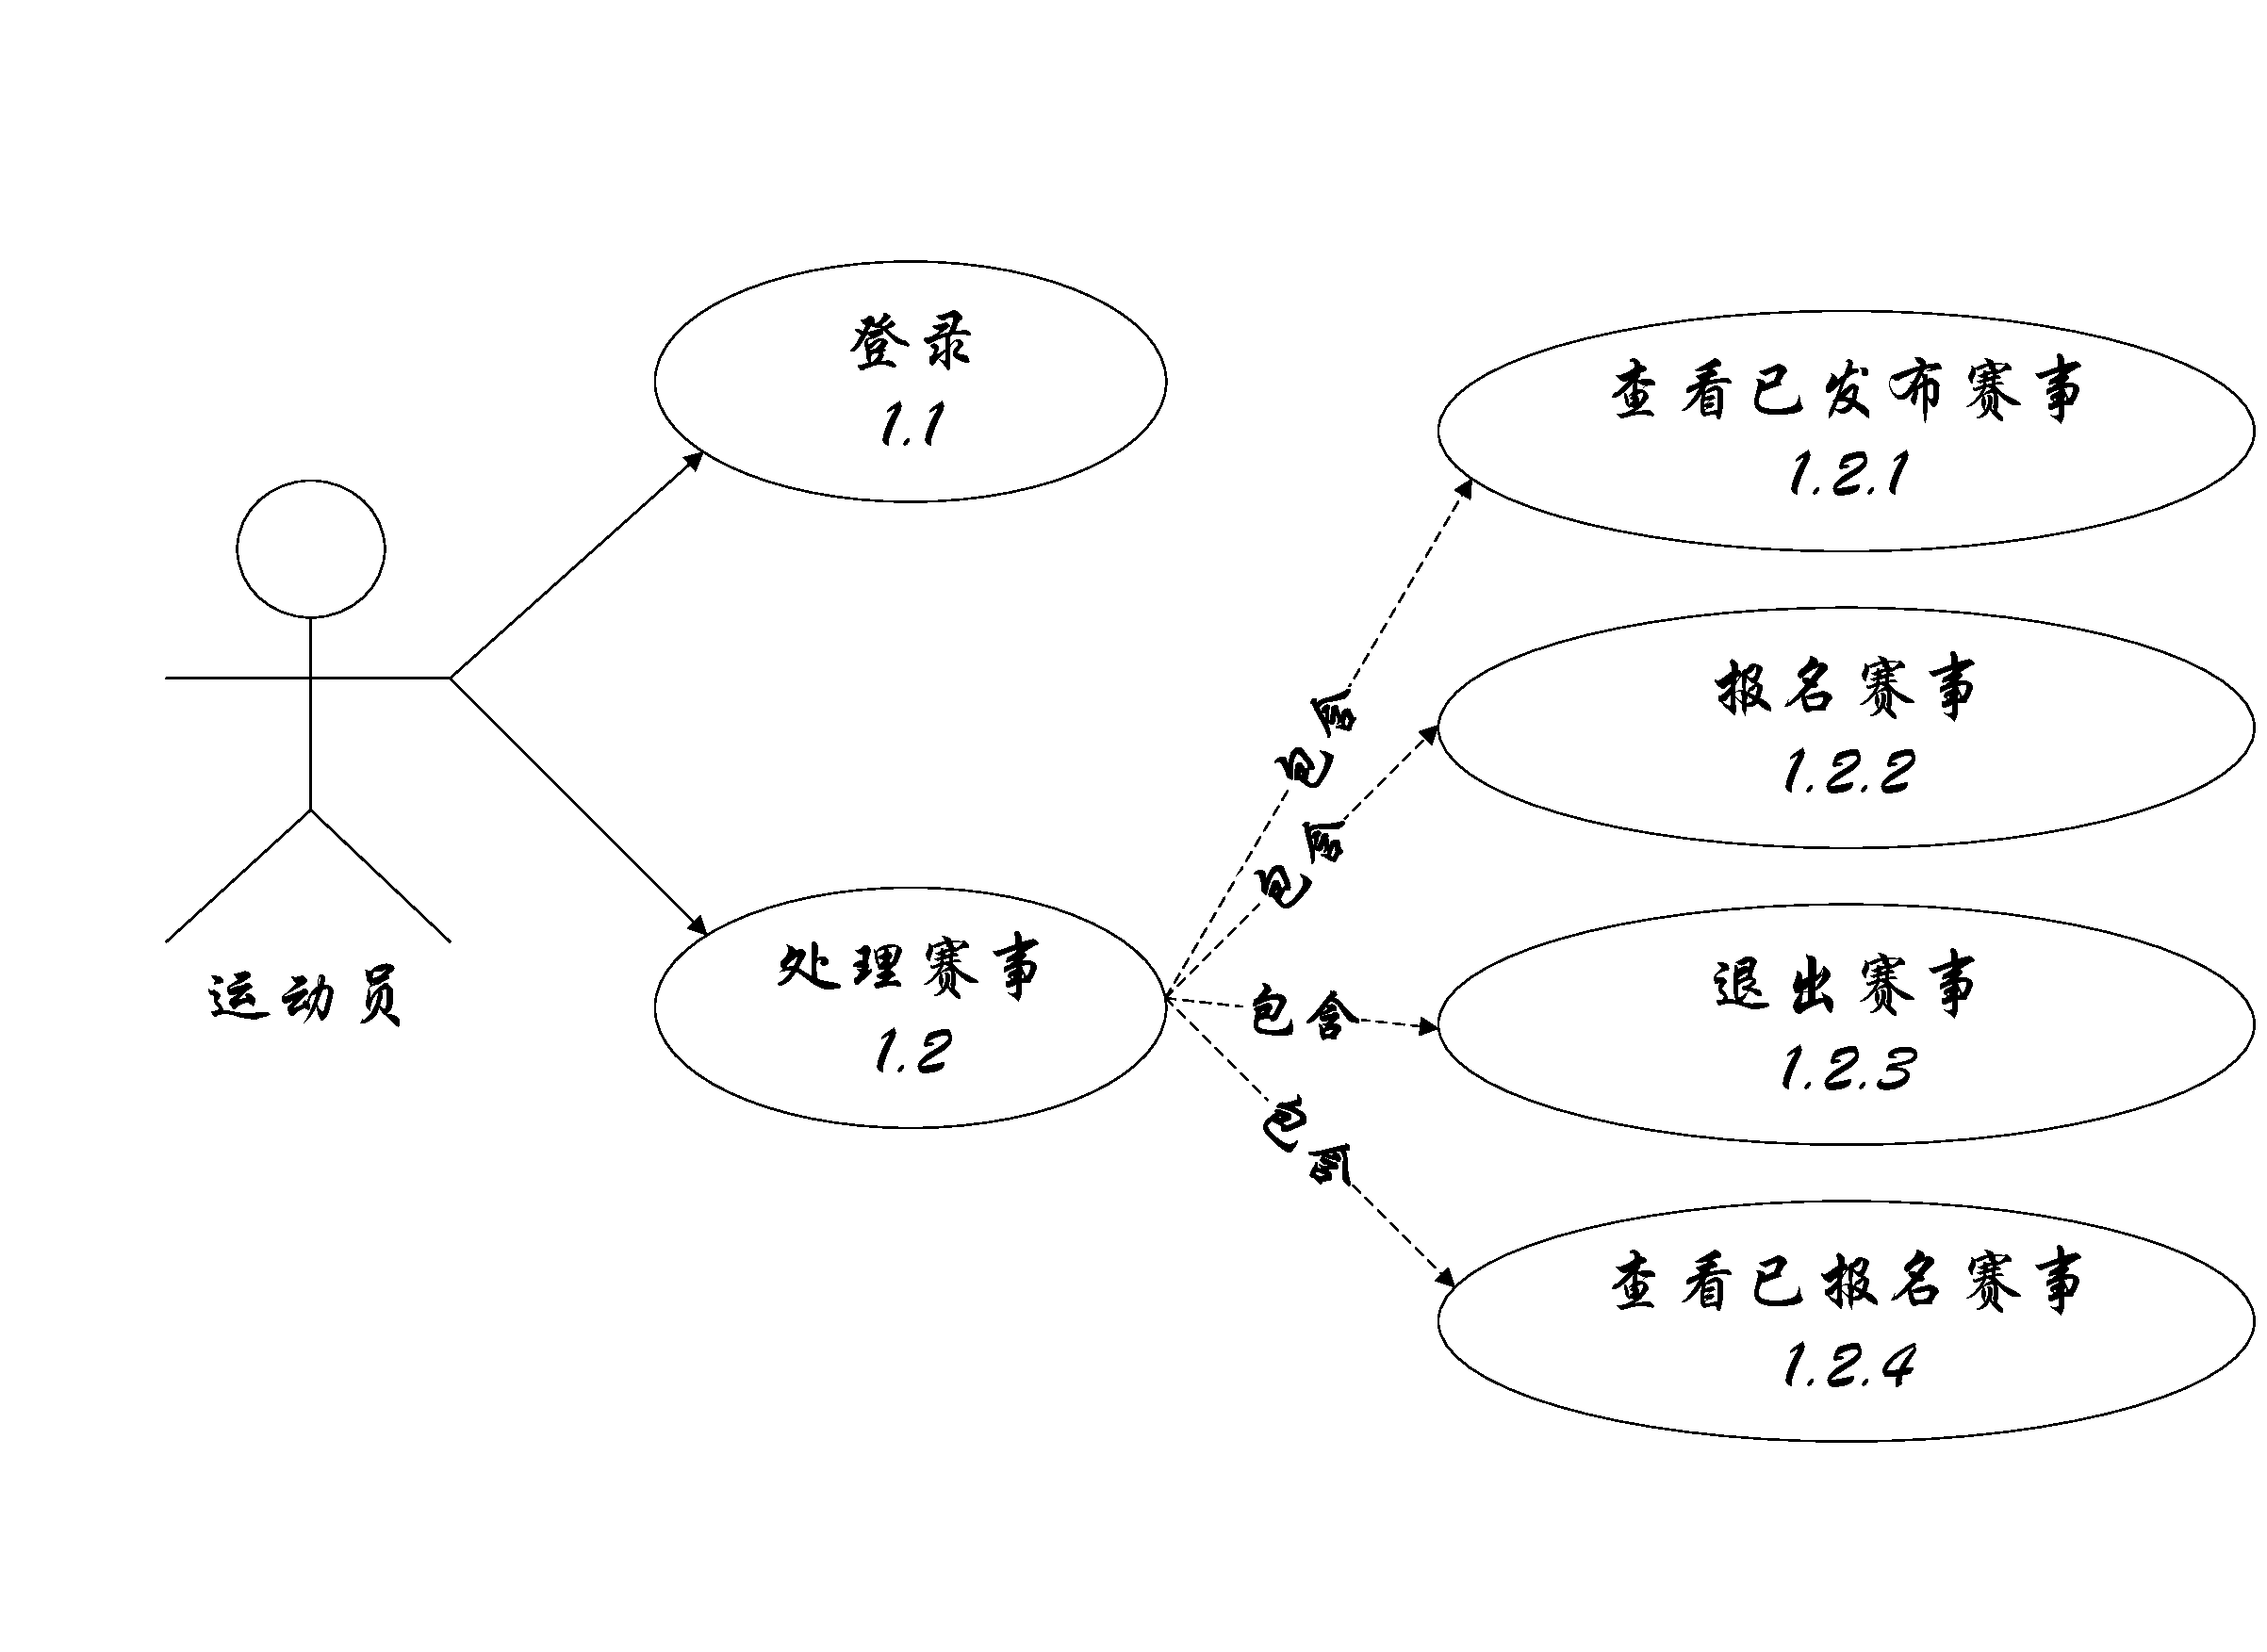
\includegraphics[width=1\columnwidth]{uc1}
	\centering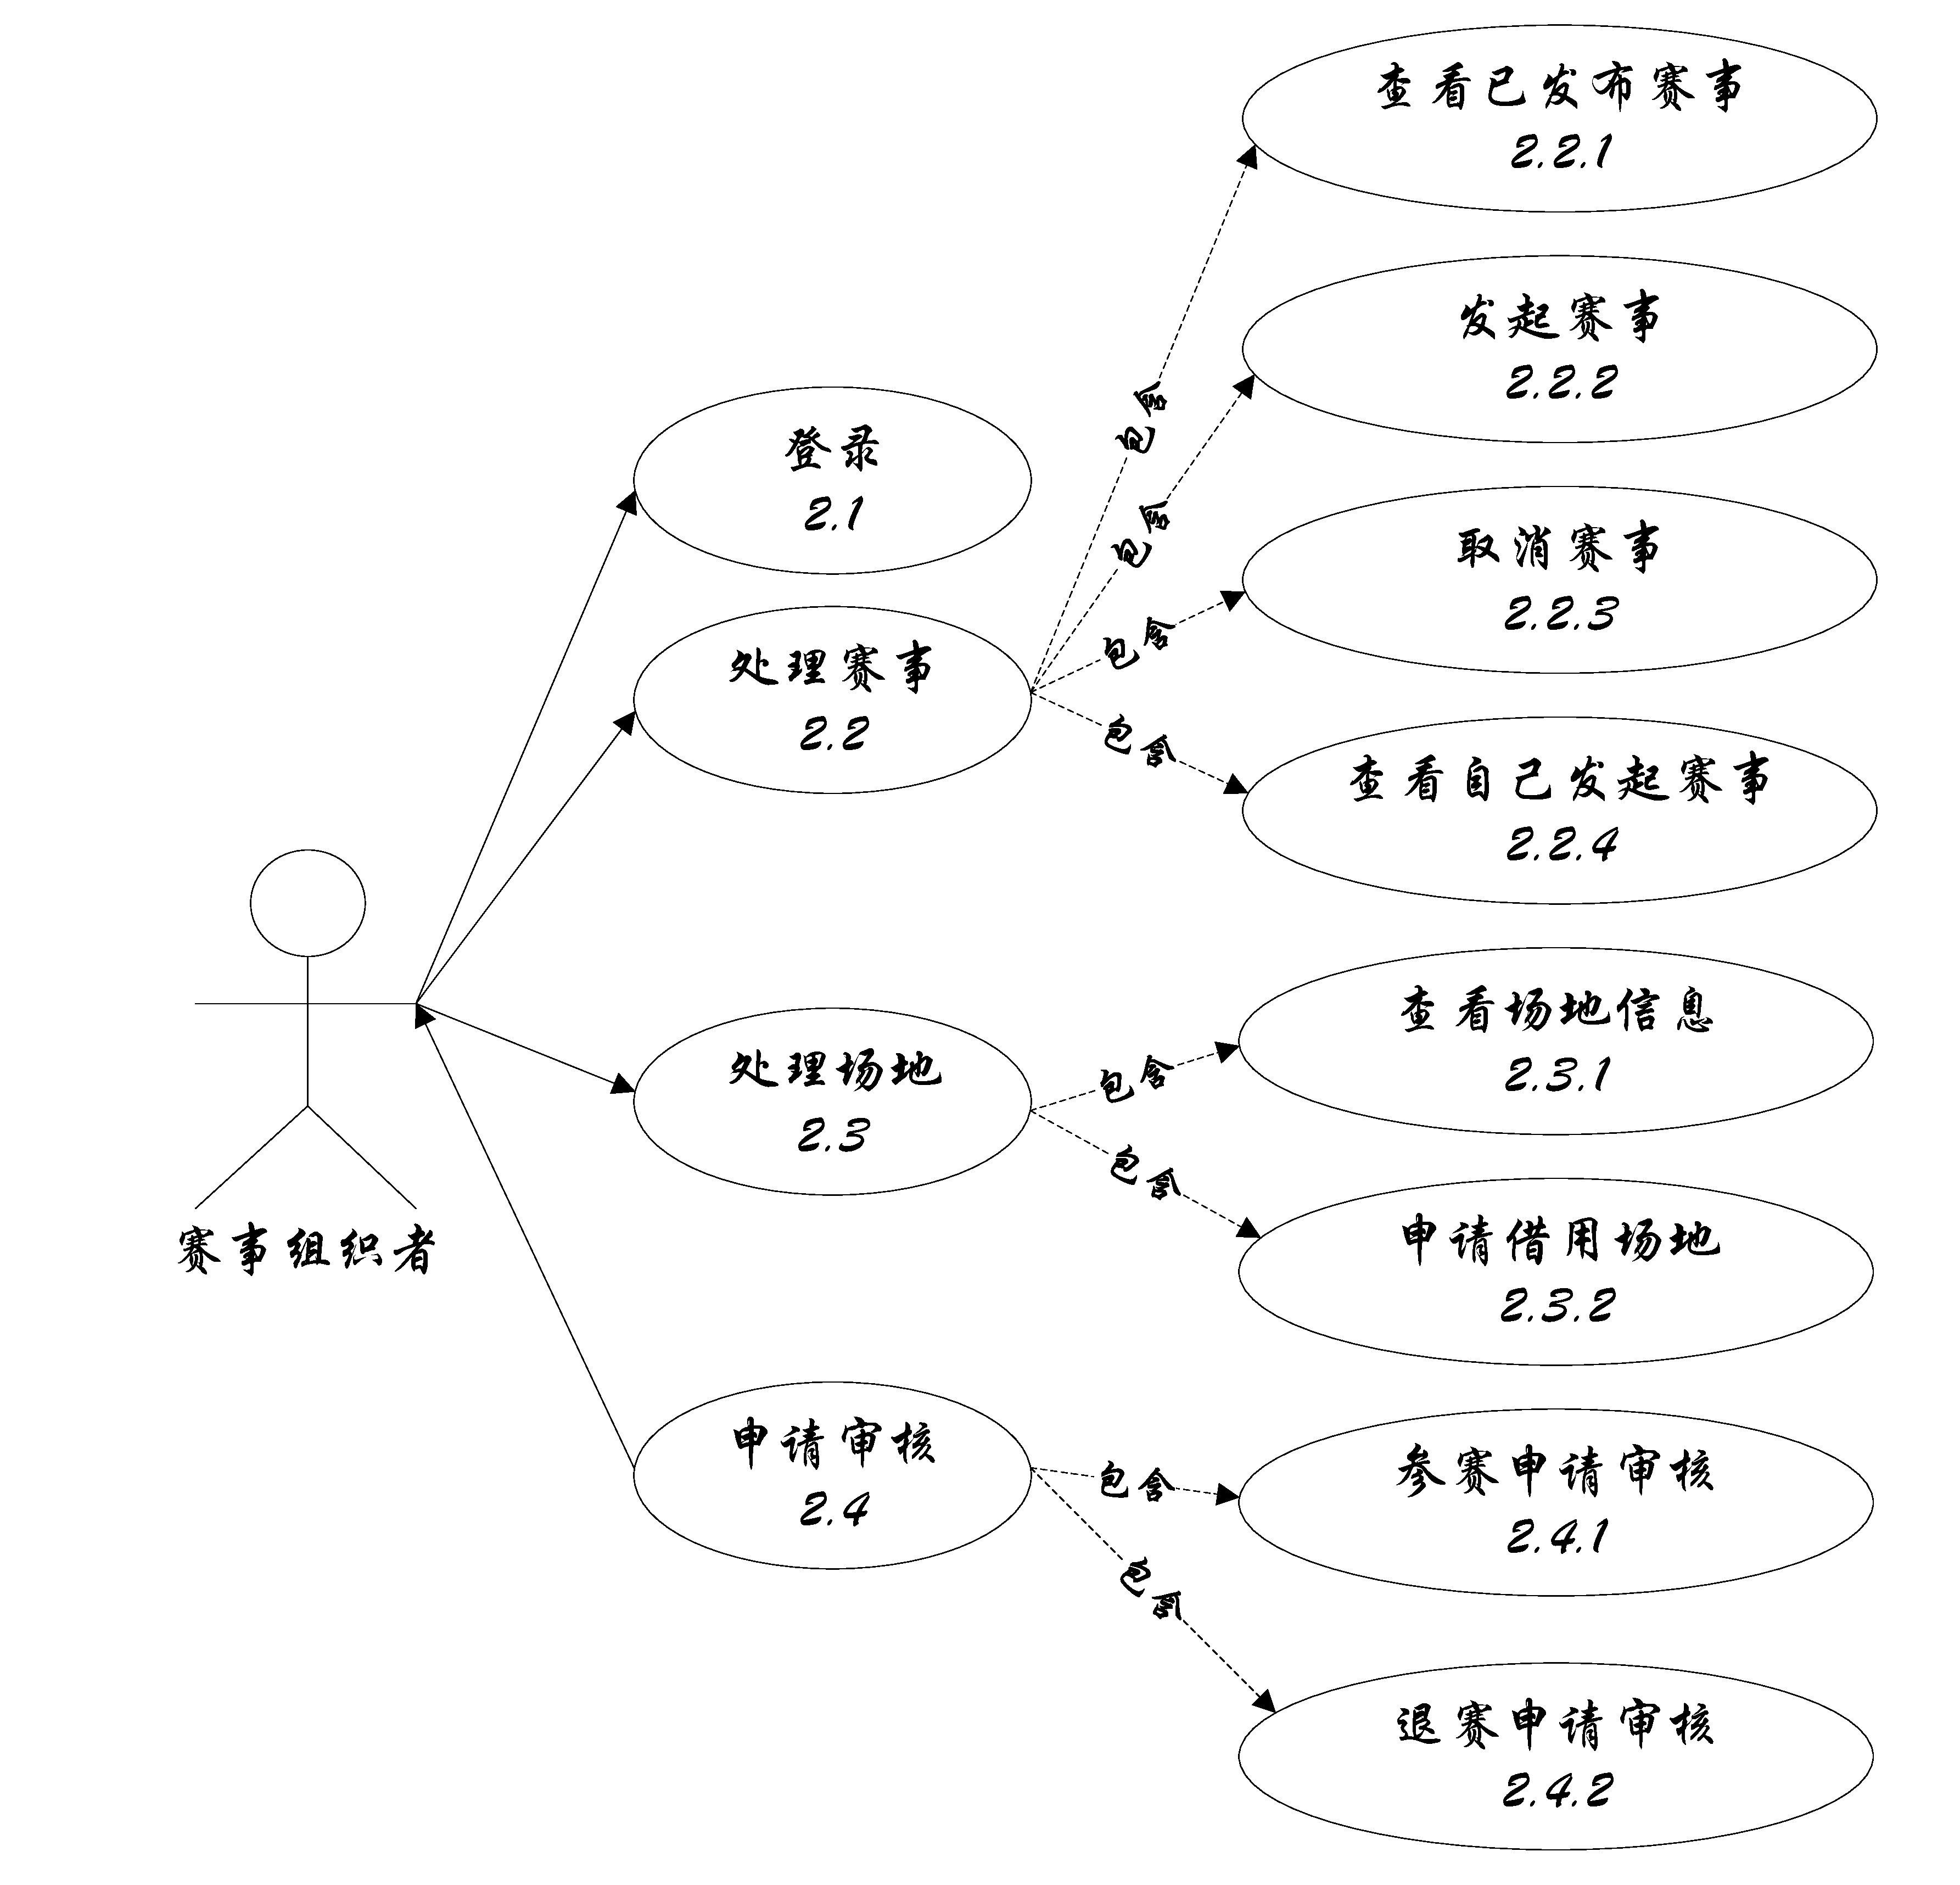
\includegraphics[width=1\columnwidth]{uc2}
	\centering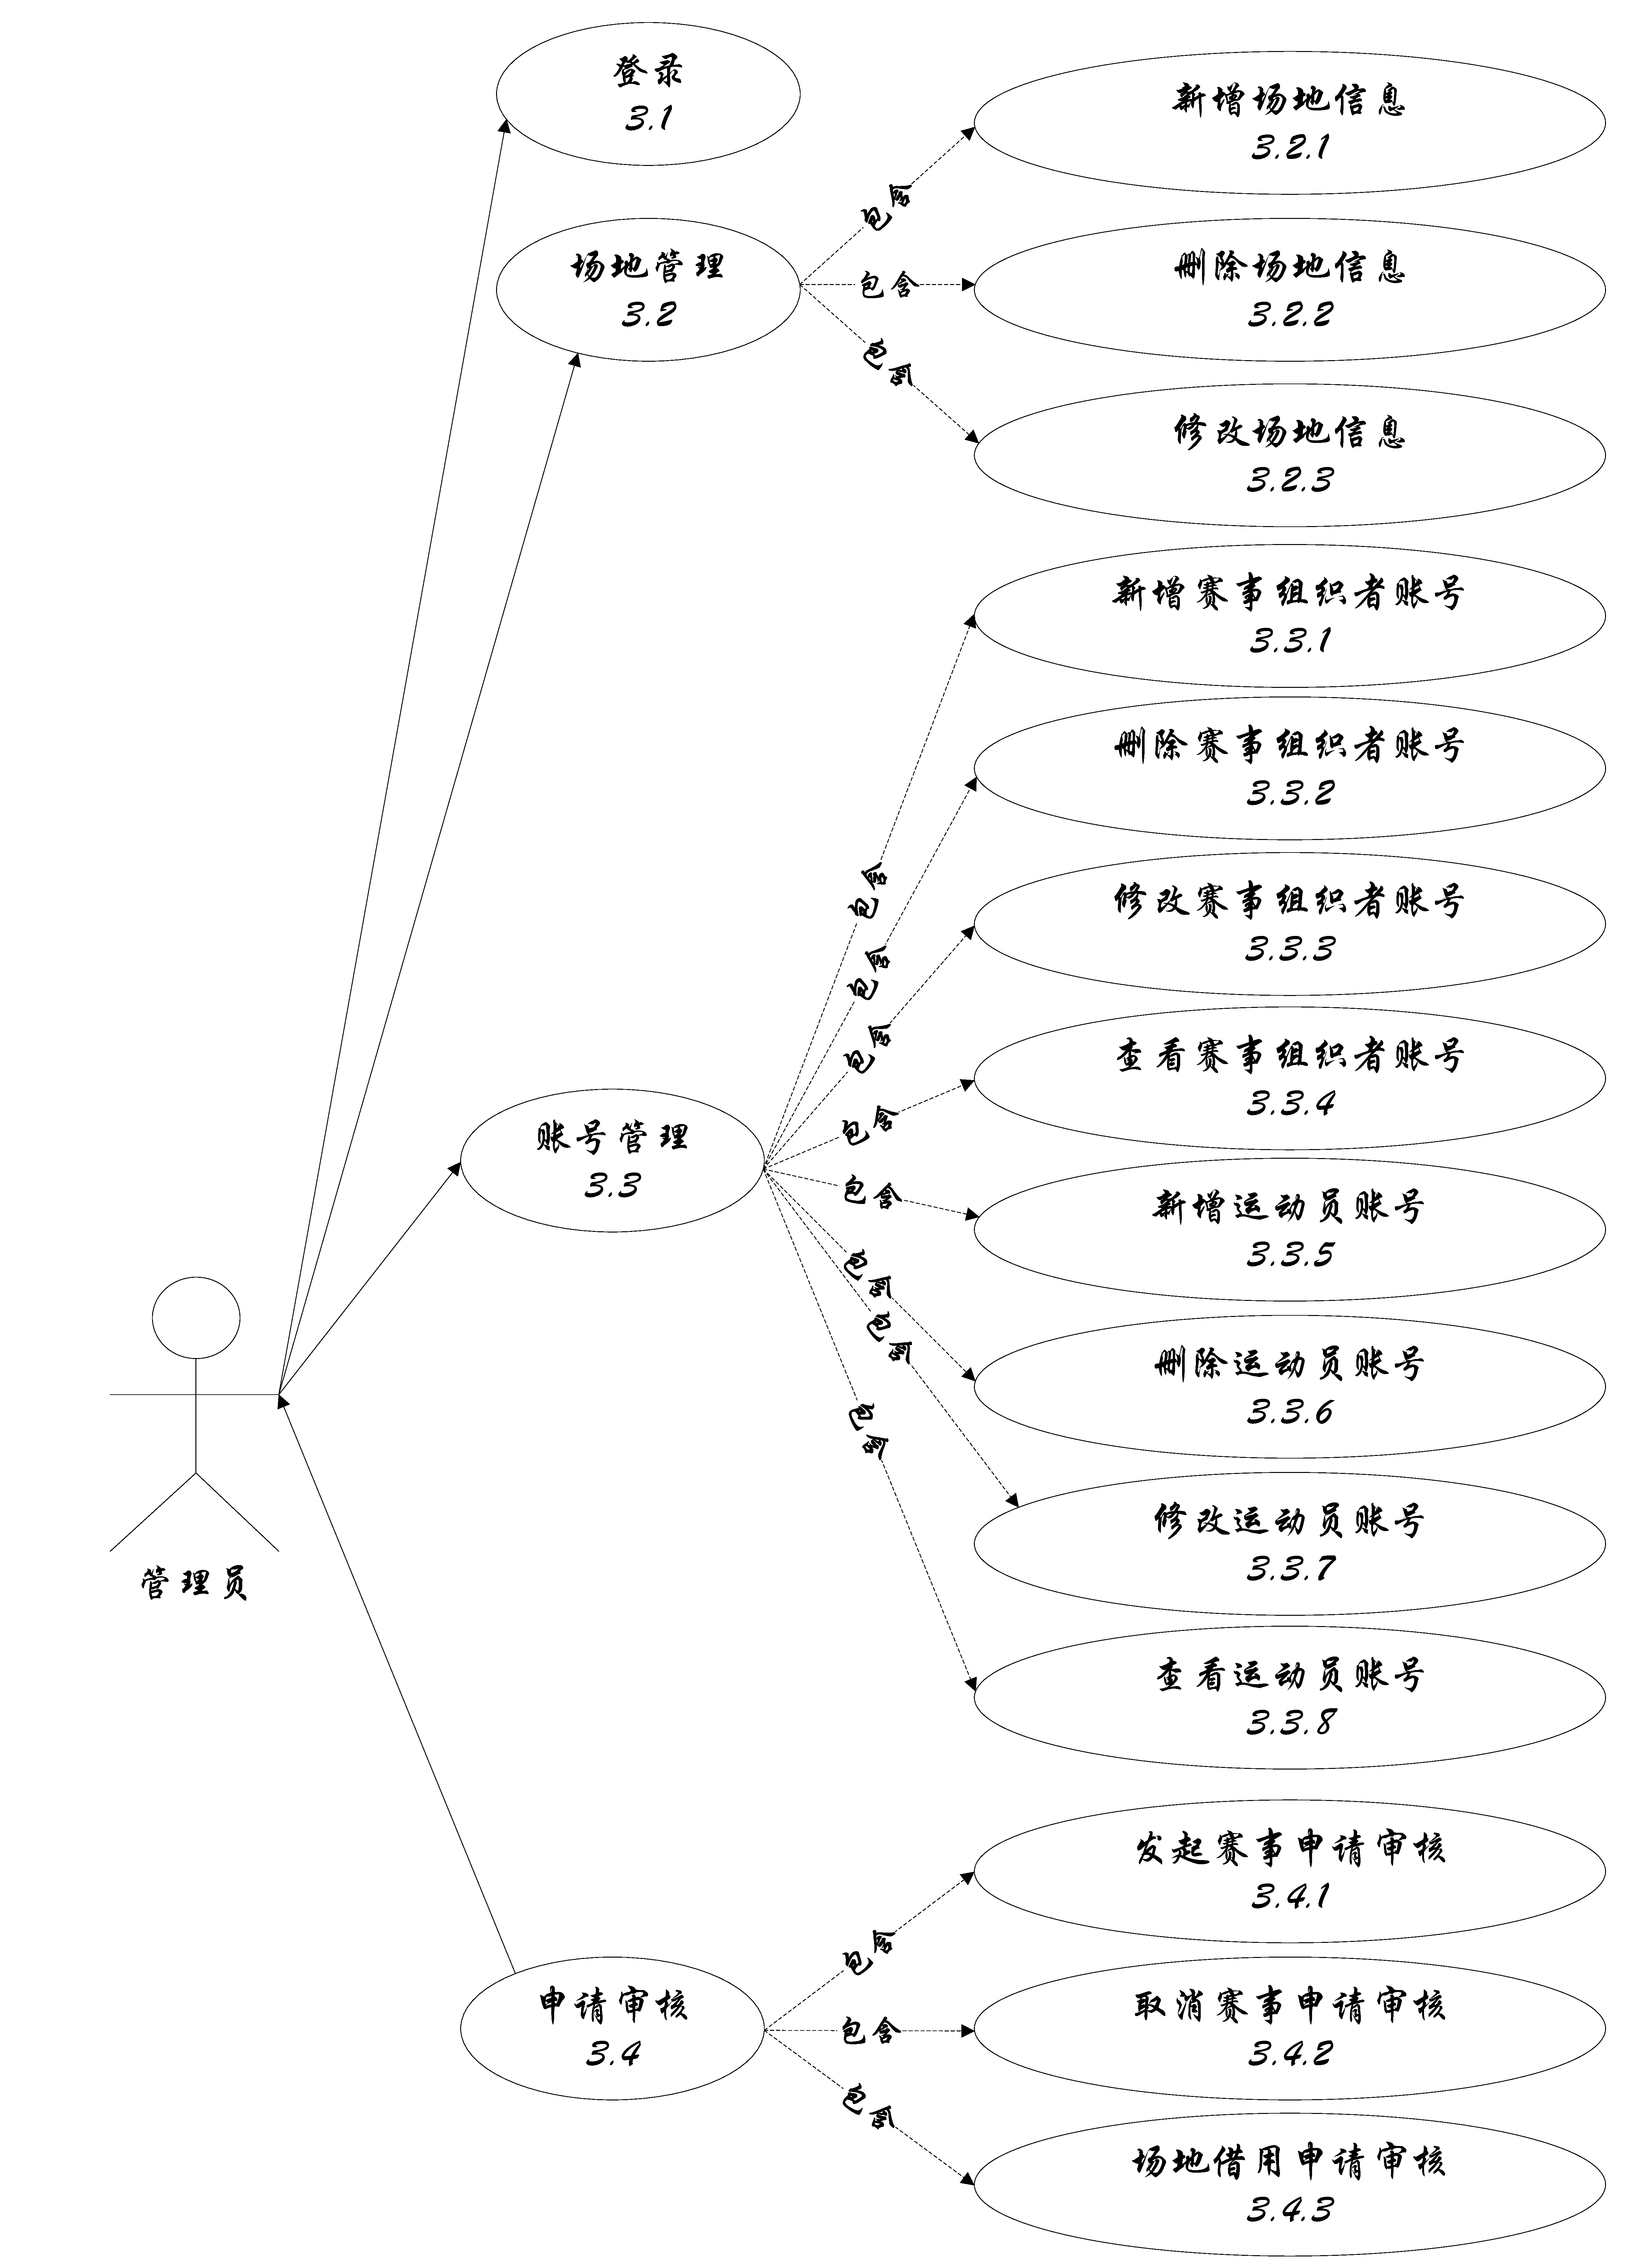
\includegraphics[width=1\columnwidth]{uc3}
	
}

\subsubsection{用例描述}

\begin{table}[H]
	\begin{center}
		\caption{用例1.1 登录}
		\label{table:Tab_uc11}
		\begin{tabular}{|p{0.15\columnwidth}|p{0.85\columnwidth}|}
			\hline\noalign{\smallskip}
			用例编号 & 1.1\\
			\hline
			用例名称 &  登录\\
			\hline
			角色 & 运动员\\
			\hline
			前置条件 & 运动员用户打开系统\\
			\hline
			基本事件流 & 1.输入账号(必填)\\& 2.输入密码(必填) \\& 3.填写完成后确认提交,提示登录成功,用例结束\\
			\hline
			异常操作流 & 当用户未输入账号或密码时,系统提示“账号或密码不能为空” \\& 当用户输入的账号错误时,系统提示“该用户不存在” \\& 当用户输入的密码错误时,系统提示“密码错误”\\
			\hline
			其他事件流 & 用户首次登录成功时,强制要求用户对初始密码进行修改,并完善个人信息,提交后方可进行后续操作,运动员用户信息包括运动员编号、姓名、性别、出生年月、联系方式,这些信息以及密码在后续操作中可以随时修改\\
			\hline
			后置条件 & 系统显示用户基本信息,包括权限等级、编号、姓名、联系方式,显示可操作的功能选项,运动员权限下为“处理赛事”选项\\
			\hline
			Author & 王子杰 \\
			\noalign{\smallskip}
			\hline
			\noalign{\smallskip}
		\end{tabular}
		\caption{用例1.2 处理赛事}
		\label{table:Tab_uc12}
		\begin{tabular}{|p{0.15\columnwidth}|p{0.85\columnwidth}|}
			\hline\noalign{\smallskip}
			用例编号 & 1.2\\
			\hline
			用例名称 &  处理赛事\\
			\hline
			角色 & 运动员\\
			\hline
			前置条件 & 运动员用户通过身份验证登录系统 \\
			\hline
			基本事件流 & 1.运动员用户选择“处理赛事”选项时,进入该用例 \\& 2.系统跳转至赛事处理页面,给出“查看已发布赛事”、“报名赛事”、“退出赛事”、“查看已报名赛事”四个选项 \\& 3.运动员用户选择需要的选项 \\& 4.系统跳转至相应界面,用例结束\\
			\hline
			异常操作流 & Null \\
			\hline
			其他事件流 & 在选择选项前,用户可随时按“返回”按钮回到主界面 \\
			\hline
			后置条件 & 系统跳转至后续界面 \\
			\hline
			Author & 王子杰 \\
			\noalign{\smallskip}
			\hline
			\noalign{\smallskip}
		\end{tabular}
	\end{center}
\end{table}

\begin{table}[H]
\begin{center}
	\caption{用例1.2.1 查看已发布赛事}
	\label{table:Tab_uc121}
	\begin{tabular}{|p{0.15\columnwidth}|p{0.85\columnwidth}|}
		\hline\noalign{\smallskip}
		用例编号 & 1.2.1\\
		\hline
		用例名称 &  查看已发布赛事\\
		\hline
		角色 & 运动员\\
		\hline
		前置条件 & 运动员用户处在赛事处理界面\\
		\hline
		基本事件流 & 1.运动员用户选择“查看已发布赛事”选项时,进入该用例 \\& 2.系统跳转至已发布赛事查询页面,无输入时,系统默认查询全部已发布的赛事信息,并返回全部已发布赛事的查询结果,每一项查询结果仅包括赛事编号和赛事名称 \\& 3.用户输入指定赛事名称或编号,罗列查询结果 \\& 4.用户选择特定的结果项查看其详细信息,详细信息仅包括赛事编号、赛事名称、赛事起止时间、赛事举办场地、赛事组织者姓名、赛事组织者联系方式、赛事说明以及赛事当前状态(预热中、进行中、已结束)\\& 5.用户按“返回”按钮,返回到处理赛事界面,用例结束\\
		\hline
		异常操作流 & 用户输入指定赛事名称或编号时,若不存在对应赛事,则对用户进行提示 \\
		\hline
		其他事件流 & Null \\
		\hline
		后置条件 & 返回到处理赛事界面\\
		\hline
		Author & 王子杰 \\
		\noalign{\smallskip}
		\hline
		\noalign{\smallskip}
	\end{tabular}
\end{center}
\end{table}

\begin{table}[!htbp]
	\begin{center}
		\caption{用例1.2.2 报名赛事}
		\label{table:Tab_uc122}
		\begin{tabular}{|p{0.15\columnwidth}|p{0.85\columnwidth}|}
			\hline\noalign{\smallskip}
			用例编号 & 1.2.2\\
			\hline
			用例名称 &  报名赛事\\
			\hline
			角色 & 运动员\\
			\hline
			前置条件 & 运动员用户处在赛事处理界面\\
			\hline
			基本事件流 & 1.运动员用户选择“报名赛事”选项时,进入该用例 \\& 2.无输入时,系统默认查询并显示全部已发布的赛事信息,每一项查询结果仅包括赛事编号和赛事名称 \\& 3.用户输入指定赛事名称或编号,罗列查询结果 \\& 4.用户选择特定的结果项查看其详细信息,详细信息仅包括赛事编号、赛事名称、赛事起止时间、赛事举办场地、赛事组织者姓名、赛事组织者联系方式、赛事说明以及赛事当前状态(预热中、进行中、已结束)\\& 5.用户按赛事详细信息最后的“报名”按钮提交报名,提示“申请提交成功,请等待赛事组织者审核”,并由系统交由赛事组织者进行审核,用例结束\\
			\hline
				异常操作流 & 用户输入指定赛事名称或编号时,若不存在对应赛事,则对用户进行提示 \\& 赛事处于进行中状态,则提示“赛事已开始 ,不可报名参赛” \\& 赛事处于已结束状态,则提示“赛事已结束 ,不可报名参赛” \\& 运动员已报名赛事时间与当前赛事冲突,则提示“当前赛事与已报名赛事时间冲突”\\
			\hline
			其他事件流 & 在提交报名申请前,用户可随时按“返回”按钮回到上一界面\\
			\hline
			后置条件 & 提示“申请提交成功,请等待赛事组织者审核”,并由系统交由赛事组织者进行审核\\
			\hline
			Author & 王子杰 \\
			\noalign{\smallskip}
			\hline
			\noalign{\smallskip}
		\end{tabular}
	\end{center}
\end{table}

\begin{table}[H]
	\begin{center}
		\caption{用例1.2.3 退出赛事}
		\label{table:Tab_uc123}
		\begin{tabular}{|p{0.15\columnwidth}|p{0.85\columnwidth}|}
			\hline\noalign{\smallskip}
			用例编号 & 1.2.3\\
			\hline
			用例名称 &  退出赛事\\
			\hline
			角色 & 运动员\\
			\hline
			前置条件 & 运动员用户处在赛事处理界面\\
			\hline
			基本事件流 & 1.运动员用户选择“退出赛事”选项时,进入该用例 \\& 2.系统查询该运动员已成功报名的赛事,返回并显示查询结果,每一项查询结果仅包括赛事编号和赛事名 \\& 3.用户按赛事详细信息最后的“退出”按钮提交退出,提示“申请提交成功,请等待赛事组织者审核”,并由系统交由赛事组织者进行审核,用例结束\\
			\hline
			异常操作流 & 查询当前用户已成功报名的赛事时,若未查询到结果,则提示“您当前尚未报名参与赛事” \\& 赛事处于进行中状态,则提示“赛事已开始 ,不可退赛” \\& 赛事处于已结束状态,则提示“赛事已结束 ,不可退赛” \\
			\hline
			其他事件流 & 在提交退赛申请前,用户可随时按“返回”按钮回到上一界面\\
			\hline
			后置条件 & 提示“申请提交成功,请等待赛事组织者审核”,并由系统交由赛事组织者进行审核\\
			\hline
			Author & 王子杰 \\
			\noalign{\smallskip}
			\hline
			\noalign{\smallskip}
		\end{tabular}
	\end{center}
\end{table}

\begin{table}[H]
	\begin{center}
		\caption{用例1.2.4 查看已报名赛事}
		\label{table:Tab_uc124}
		\begin{tabular}{|p{0.15\columnwidth}|p{0.85\columnwidth}|}
			\hline\noalign{\smallskip}
			用例编号 & 1.2.4\\
			\hline
			用例名称 & 查看已报名赛事\\
			\hline
			角色 & 运动员\\
			\hline
			前置条件 & 运动员用户处在赛事处理界面\\
			\hline
			基本事件流 & 1.运动员用户选择“查看已报名赛事”选项时,进入该用例 \\& 2.系统查询该运动员已成功报名的赛事,返回并显示查询结果,每一项查询结果仅包括赛事编号和赛事名 \\& 3.用户选择特定的结果项查看其详细信息,详细信息仅包括赛事编号、赛事名称、赛事起止时间、赛事举办场地、赛事组织者姓名、赛事组织者联系方式、赛事说明以及赛事当前状态(预热中、进行中、已结束)\\& 4.用户按“返回”按钮,返回到处理赛事界面,用例结束\\
			\hline
			异常操作流 & 查询当前用户已成功报名的赛事时,若未查询到结果,则提示“您当前尚未报名参与赛事”  \\
			\hline
			其他事件流 & Null\\
			\hline
			后置条件 & 返回到处理赛事界面\\
			\hline
			Author & 王子杰 \\
			\noalign{\smallskip}
			\hline
			\noalign{\smallskip}
		\end{tabular}
	%\end{center}
	%\begin{center}
	\caption{用例2.1 登录}
	\label{table:Tab_uc21}
	\begin{tabular}{|p{0.15\columnwidth}|p{0.85\columnwidth}|}
		\hline\noalign{\smallskip}
		用例编号 & 2.1\\
		\hline
		用例名称 &  登录\\
		\hline
		角色 & 赛事组织者\\
		\hline
		前置条件 & 赛事组织者用户打开系统\\
		\hline
		基本事件流 & 1.输入账号(必填)\\& 2.输入密码(必填) \\& 3.填写完成后确认提交,提示登录成功,用例结束\\
		\hline
		异常操作流 & 当用户未输入账号或密码时,系统提示“账号或密码不能为空” \\& 当用户输入的账号错误时,系统提示“该用户不存在” \\& 当用户输入的密码错误时,系统提示“密码错误”\\
		\hline
		其他事件流 & 用户首次登录成功时,强制要求用户对初始密码进行修改,并完善个人信息,提交后方可进行后续操作,赛事组织者信息包括组织者编号、姓名、联系方式,这些信息以及密码在后续操作中可以随时修改\\
		\hline
		后置条件 & 系统显示用户基本信息,包括权限等级、编号、姓名、联系方式,显示可操作的功能选项,赛事组织者权限下为“处理赛事”,“处理场地”,“申请审核”选项\\
		\hline
		Author & 王子杰 \\
		\noalign{\smallskip}
		\hline
		\noalign{\smallskip}
	\end{tabular}
\end{center}
\end{table}

\begin{table}[H]
	\begin{center}
		\caption{用例2.2 处理赛事}
		\label{table:Tab_uc22}
		\begin{tabular}{|p{0.15\columnwidth}|p{0.85\columnwidth}|}
			\hline\noalign{\smallskip}
			用例编号 & 2.2\\
			\hline
			用例名称 &  处理赛事\\
			\hline
			角色 & 赛事组织者\\
			\hline
			前置条件 & 赛事组织者用户通过身份验证登录系统 \\
			\hline
			基本事件流 & 1.赛事组织者用户选择“处理赛事”选项时,进入该用例 \\& 2.系统跳转至赛事处理页面,给出“查看已发布赛事”、“发起赛事”、“取消赛事”、“查看自己发起赛事”四个选项 \\& 3.赛事组织者用户选择需要的选项 \\& 4.系统跳转至相应界面,用例结束\\
			\hline
			异常操作流 & Null \\
			\hline
			其他事件流 & 在选择选项前,用户可随时按“返回”按钮回到主界面 \\
			\hline
			后置条件 & 系统跳转至后续界面 \\
			\hline
			Author & 王子杰 \\
			\noalign{\smallskip}
			\hline
			\noalign{\smallskip}
		\end{tabular}
		\caption{用例2.2.1 查看已发布赛事}
		\label{table:Tab_uc221}
		\begin{tabular}{|p{0.15\columnwidth}|p{0.85\columnwidth}|}
			\hline\noalign{\smallskip}
			用例编号 & 2.2.1\\
			\hline
			用例名称 &  查看已发布赛事\\
			\hline
			角色 & 赛事组织者\\
			\hline
			前置条件 & 赛事组织者用户处在赛事处理界面\\
			\hline
			基本事件流 & 1.赛事组织者用户选择“查看已发布赛事”选项时,进入该用例 \\& 2.系统跳转至已发布赛事查询页面,无输入时,系统默认查询全部已发布的赛事信息,并返回全部已发布赛事的查询结果,每一项查询结果仅包括赛事编号和赛事名称 \\& 3.用户输入指定赛事名称或编号,罗列查询结果 \\& 4.用户选择特定的结果项查看其详细信息,详细信息仅包括赛事编号、赛事名称、赛事起止时间、赛事举办场地、赛事组织者姓名、赛事组织者联系方式、赛事说明以及赛事当前状态(预热中、进行中、已结束)\\& 5.用户按“返回”按钮,返回到处理赛事界面,用例结束\\
			\hline
			异常操作流 & 用户输入指定赛事名称或编号时,若不存在对应赛事,则对用户进行提示 \\
			\hline
			其他事件流 & Null \\
			\hline
			后置条件 & 返回到处理赛事界面\\
			\hline
			Author & 王子杰 \\
			\noalign{\smallskip}
			\hline
			\noalign{\smallskip}
		\end{tabular}
	\end{center}
\end{table}

\begin{table}[H]
	\begin{center}
		\caption{用例2.2.2 发起赛事}
		\label{table:Tab_uc222}
		\begin{tabular}{|p{0.15\columnwidth}|p{0.85\columnwidth}|}
			\hline\noalign{\smallskip}
			用例编号 & 2.2.2\\
			\hline
			用例名称 &  发起赛事\\
			\hline
			角色 & 赛事组织者\\
			\hline
			前置条件 & 赛事组织者用户处在赛事处理界面\\
			\hline
			基本事件流 & 1.赛事组织者用户选择“发起赛事”选项时,进入该用例 \\& 2.选择赛事举办场地\\& 3.选择起止时间 \\& 4.填写赛事名称 \\& 5.填写赛事说明\\& 6.赛事组织者用户按“发起赛事”按钮”提交申请,提示“赛事发起申请提交成功,请等待管理员审核” ,并由系统交由管理员进行审核,用例结束\\
			\hline
			异常操作流 & 所选时段场地未成功借用,则提示“所选时段该场地未成功申请借用” \\& 相关信息未填写完整,则提示“请完善赛事信息”\\
			\hline
			其他事件流 & 在提交报名申请前,用户可随时按“返回”按钮回到上一界面\\
			\hline
			后置条件 & 提示“赛事发起申请提交成功,请等待管理员审核” ,并由系统交由管理员进行审核\\
			\hline
			Author & 王子杰 \\
			\noalign{\smallskip}
			\hline
			\noalign{\smallskip}
		\end{tabular}
	\end{center}
\end{table}

\begin{table}[H]
	\begin{center}
		\caption{用例2.2.3 取消赛事}
		\label{table:Tab_uc223}
		\begin{tabular}{|p{0.15\columnwidth}|p{0.85\columnwidth}|}
			\hline\noalign{\smallskip}
			用例编号 & 2.2.3\\
			\hline
			用例名称 &  取消赛事\\
			\hline
			角色 & 赛事组织者\\
			\hline
			前置条件 & 赛事组织者用户处在赛事处理界面\\
			\hline
			基本事件流 & 1.赛事组织者用户选择“取消赛事”选项时,进入该用例 \\& 2.查询当前用户已成功发起的赛事,返回并显示查询结果,每一项查询结果仅包括赛事编号和赛事名称 \\& 3.用户按赛事信息最后的“取消赛事”按钮提交取消申请,提示“赛事取消申请提交成功,请等待管理员审核”,并由系统交由管理员进行审核,用例结束\\
			\hline
			异常操作流 & 查询当前用户已成功发起的赛事时,若未查询到结果,则提示“您当前尚未报名参与赛事” \\& 赛事处于进行中状态,则提示“赛事已开始 ,不可取消” \\& 赛事处于已结束状态,则提示“赛事已结束 ,不可取消” \\
			\hline
			其他事件流 & 在提交取消赛事申请前,用户可随时按“返回”按钮回到上一界面\\
			\hline
			后置条件 & 提示“赛事取消申请提交成功,请等待管理员审核”,并由系统交由管理员进行审核\\
			\hline
			Author & 王子杰 \\
			\noalign{\smallskip}
			\hline
			\noalign{\smallskip}
		\end{tabular}
	\end{center}
\end{table}

\begin{table}[H]
	\begin{center}
		\caption{用例2.2.4 查看自己发起赛事}
		\label{table:Tab_uc224}
		\begin{tabular}{|p{0.15\columnwidth}|p{0.85\columnwidth}|}
			\hline\noalign{\smallskip}
			用例编号 & 2.2.4\\
			\hline
			用例名称 & 查看自己发起赛事\\
			\hline
			角色 & 赛事组织者\\
			\hline
			前置条件 & 赛事组织者用户处在赛事处理界面\\
			\hline
			基本事件流 & 1.赛事组织者用户选择“查看自己发起赛事”选项时,进入该用例 \\& 2.查询当前用户已成功发起的赛事,返回并显示查询结果,每一项查询结果仅包括赛事编号和赛事名称 \\& 3.用户选择特定的结果项查看其详细信息,详细信息仅包括赛事编号、赛事名称、赛事起止时间、赛事举办场地、赛事组织者姓名、赛事组织者联系方式、赛事说明以及赛事当前状态(预热中、进行中、已结束)\\& 4.用户按“返回”按钮,返回到处理赛事界面,用例结束\\
			\hline
			异常操作流 & 查询当前用户已成功发起的赛事时,若未查询到结果,则提示“您当前尚未报名参与赛事”  \\
			\hline
			其他事件流 & Null\\
			\hline
			后置条件 & 返回到处理赛事界面\\
			\hline
			Author & 王子杰 \\
			\noalign{\smallskip}
			\hline
			\noalign{\smallskip}
		\end{tabular}
		\caption{用例2.3 处理场地}
		\label{table:Tab_uc23}
		\begin{tabular}{|p{0.15\columnwidth}|p{0.85\columnwidth}|}
			\hline\noalign{\smallskip}
			用例编号 & 2.3\\
			\hline
			用例名称 &  处理场地\\
			\hline
			角色 & 赛事组织者\\
			\hline
			前置条件 & 赛事组织者用户通过身份验证登录系统 \\
			\hline
			基本事件流 & 1.赛事组织者用户选择“处理场地”选项时,进入该用例 \\& 2.系统跳转至场地处理页面,给出“查看场地信息”、“申请借用场地”两个选项 \\& 3.赛事组织者用户选择需要的选项 \\& 4.系统跳转至相应界面,用例结束\\
			\hline
			异常操作流 & Null \\
			\hline
			其他事件流 & 在选择选项前,用户可随时按“返回”按钮回到主界面 \\
			\hline
			后置条件 & 系统跳转至后续界面 \\
			\hline
			Author & 王子杰 \\
			\noalign{\smallskip}
			\hline
			\noalign{\smallskip}
		\end{tabular}
	\end{center}
\end{table}


\begin{table}[H]
	\begin{center}
		\caption{用例2.3.1 查看场地信息}
		\label{table:Tab_uc231}
		\begin{tabular}{|p{0.15\columnwidth}|p{0.85\columnwidth}|}
			\hline\noalign{\smallskip}
			用例编号 & 2.3.1\\
			\hline
			用例名称 &  查看场地信息\\
			\hline
			角色 & 赛事组织者\\
			\hline
			前置条件 & 赛事组织者用户处在场地处理界面\\
			\hline
			基本事件流 & 1.赛事组织者用户选择“查看场地信息”选项时,进入该用例 \\& 2.系统跳转至场地信息查询页面,无输入时,系统默认查询全部场地信息,并返回全部场地信息的查询结果,每一项查询结果仅包括场地编号和场地名称 \\& 3.用户输入指定场地名称、编号或空闲时间段,罗列查询结果 \\& 4.用户选择特定的结果项查看其详细信息,详细信息仅包括场地编号、场地名称、地址、场地空闲时间段 \\& 5.用户按“返回”按钮,返回到处理赛事界面,用例结束\\
			\hline
			异常操作流 & 用户输入指定场地名称、编号或空闲时间段时,若不存在对应场地,则对用户进行提示 \\
			\hline
			其他事件流 & Null \\
			\hline
			后置条件 & 返回到处理赛事界面\\
			\hline
			Author & 王子杰 \\
			\noalign{\smallskip}
			\hline
			\noalign{\smallskip}
		\end{tabular}
	\end{center}
\end{table}
			
\begin{table}[H]
	\begin{center}
		\caption{用例2.3.2 申请借用场地}
		\label{table:Tab_uc232}
		\begin{tabular}{|p{0.15\columnwidth}|p{0.85\columnwidth}|}
			\hline\noalign{\smallskip}
			用例编号 & 2.3.2\\
			\hline
			用例名称 &  申请借用场地\\
			\hline
			角色 & 赛事组织者\\
			\hline
			前置条件 & 赛事组织者用户处在场地处理界面\\
			\hline
			基本事件流 & 1.赛事组织者用户选择“申请借用场地”选项时,进入该用例 \\& 2.无输入时,系统默认查询全部场地信息,并返回全部场地信息的查询结果,每一项查询结果仅包括场地编号和场地名称 \\& 3.用户输入指定场地名称、编号或空闲时间段,罗列查询结果 \\& 4.用户选择特定的结果项查看其详细信息,详细信息仅包括场地编号、场地名称、地址、场地空闲时间段 \\& 5.用户按场地详细信息最后的“申请借用”按钮\\& 6.选择要借用的场地编号与借用起止时间,借用时长以半天为最小单位 \\& 7.填写场地借用说明 \\& 8.提交场地借用申请,提示“场地借用申请提交成功,请等待管理员审核”,由系统交由管理员进行审核,用例结束 \\
			\hline
			异常操作流 & 用户输入指定场地名称、编号或空闲时间段时,若不存在对应场地,则对用户进行提示  \\& 若所选时间段已被占用,则提示“所选时间段已被占用”\\
			\hline
			其他事件流 & 在场地借用申请前,用户可随时按“返回”按钮回到上一界面\\
			\hline
			后置条件 & 提示“场地借用申请提交成功,请等待管理员审核”,由系统交由管理员进行审核\\
			\hline
			Author & 王子杰 \\
			\noalign{\smallskip}
			\hline
			\noalign{\smallskip}
		\end{tabular}
	\end{center}
\end{table}

\begin{table}[H]
	\begin{center}
		\caption{用例2.4 申请审核}
		\label{table:Tab_uc24}
		\begin{tabular}{|p{0.15\columnwidth}|p{0.85\columnwidth}|}
			\hline\noalign{\smallskip}
			用例编号 & 2.4\\
			\hline
			用例名称 &  申请审核\\
			\hline
			角色 & 赛事组织者\\
			\hline
			前置条件 & 赛事组织者用户通过身份验证登录系统 \\
			\hline
			基本事件流 & 1.赛事组织者用户选择“申请审核”选项时,进入该用例 \\& 2.系统跳转至申请审核页面,给出“参赛申请审核”、“退赛申请审核”两个选项 \\& 3.赛事组织者用户选择需要的选项 \\& 4.系统跳转至相应界面,用例结束\\
			\hline
			异常操作流 & Null \\
			\hline
			其他事件流 & 在选择选项前,用户可随时按“返回”按钮回到主界面 \\
			\hline
			后置条件 & 系统跳转至后续界面 \\
			\hline
			Author & 王子杰 \\
			\noalign{\smallskip}
			\hline
			\noalign{\smallskip}
		\end{tabular}
		\caption{用例2.4.1 参赛申请审核}
		\label{table:Tab_uc241}
		\begin{tabular}{|p{0.15\columnwidth}|p{0.85\columnwidth}|}
			\hline\noalign{\smallskip}
			用例编号 & 2.4.1\\
			\hline
			用例名称 &  参赛申请审核\\
			\hline
			角色 & 赛事组织者\\
			\hline
			前置条件 & 赛事组织者用户处在申请审核界面 \\
			\hline
			基本事件流 & 1.赛事组织者用户选择“参赛申请审核”选项时,进入该用例 \\& 2.系统跳转至参赛申请审核页面,罗列出待处理的参赛申请,显示相应赛事的赛事编号、赛事名称,以及相应运动员的运动员编号、姓名、性别、出生年月 \\& 3.赛事组织者用户选择“同意”或“拒绝”选项后提交,若选择拒绝,可以选择附加说明信息一同反馈给运动员,提交成功后提示“审核意见提交成功” \\& 4.用户按“返回”按钮,返回到处理赛事界面,用例结束\\
			\hline
			异常操作流 & Null \\
			\hline
			其他事件流 & Null \\
			\hline
			后置条件 & 提交成功后提示“审核意见提交成功”,并将审核意见由系统反馈给运动员和赛事组织者\\& 系统跳转至上一界面 \\
			\hline
			Author & 王子杰 \\
			\noalign{\smallskip}
			\hline
			\noalign{\smallskip}
		\end{tabular}
	\end{center}
\end{table}

\begin{table}[H]
	\begin{center}
		\caption{用例2.4.2 退赛申请审核}
		\label{table:Tab_uc242}
		\begin{tabular}{|p{0.15\columnwidth}|p{0.85\columnwidth}|}
			\hline\noalign{\smallskip}
			用例编号 & 2.4.2\\
			\hline
			用例名称 &  退赛申请审核\\
			\hline
			角色 & 赛事组织者\\
			\hline
			前置条件 & 赛事组织者用户处在申请审核界面 \\
			\hline
			基本事件流 & 1.赛事组织者用户选择“退赛申请审核”选项时,进入该用例 \\& 2.系统跳转至退赛申请审核页面,罗列出待处理的退赛申请,显示相应赛事的赛事编号、赛事名称,以及相应运动员的运动员编号、姓名、性别、出生年月 \\& 3.赛事组织者用户选择“同意”或“拒绝”选项后提交,若选择拒绝,可以选择附加说明信息一同反馈给运动员,提交成功后提示“审核意见提交成功” \\& 4.用户按“返回”按钮,返回到处理赛事界面,用例结束\\
			\hline
			异常操作流 & Null \\
			\hline
			其他事件流 & Null \\
			\hline
			后置条件 & 提交成功后提示“审核意见提交成功”,并将审核意见由系统反馈给运动员和赛事组织者\\& 系统跳转至上一界面 \\
			\hline
			Author & 王子杰 \\
			\noalign{\smallskip}
			\hline
			\noalign{\smallskip}
		\end{tabular}
		\caption{用例3.1 登录}
		\label{table:Tab_uc31}
		\begin{tabular}{|p{0.15\columnwidth}|p{0.85\columnwidth}|}
			\hline\noalign{\smallskip}
			用例编号 & 3.1\\
			\hline
			用例名称 &  登录\\
			\hline
			角色 & 管理员\\
			\hline
			前置条件 & 管理员用户打开系统\\
			\hline
			基本事件流 & 1.输入账号(必填)\\& 2.输入密码(必填) \\& 3.填写完成后确认提交,提示登录成功,用例结束\\
			\hline
			异常操作流 & 当用户未输入账号或密码时,系统提示“账号或密码不能为空” \\& 当用户输入的账号错误时,系统提示“该用户不存在” \\& 当用户输入的密码错误时,系统提示“密码错误”\\
			\hline
			其他事件流 & Null\\
			\hline
			后置条件 & 系统显示用户基本信息,包括权限等级、编号、姓名、联系方式,显示可操作的功能选项,管理员权限下为“场地管理”,“账号管理”,“申请审核”选项\\
			\hline
			Author & 王子杰 \\
			\noalign{\smallskip}
			\hline
			\noalign{\smallskip}
		\end{tabular}
	\end{center}
\end{table}

\begin{table}[H]
	\begin{center}
		\caption{用例3.2 场地管理}
		\label{table:Tab_uc32}
		\begin{tabular}{|p{0.15\columnwidth}|p{0.85\columnwidth}|}
			\hline\noalign{\smallskip}
			用例编号 & 3.2\\
			\hline
			用例名称 &  场地管理\\
			\hline
			角色 & 管理员\\
			\hline
			前置条件 & 管理员用户通过身份验证登录系统 \\
			\hline
			基本事件流 & 1.管理员用户选择“场地管理”选项时,进入该用例 \\& 2.系统跳转至场地管理页面,给出“新增场地信息”、“删除场地信息”、“修改场地信息”三个选项 \\& 3.管理员用户选择需要的选项 \\& 4.系统跳转至相应界面,用例结束\\
			\hline
			异常操作流 & Null \\
			\hline
			其他事件流 & 在选择选项前,用户可随时按“返回”按钮回到主界面 \\
			\hline
			后置条件 & 系统跳转至后续界面 \\
			\hline
			Author & 王子杰 \\
			\noalign{\smallskip}
			\hline
			\noalign{\smallskip}
		\end{tabular}
		\caption{用例3.2.1 新增场地信息}
		\label{table:Tab_uc321}
		\begin{tabular}{|p{0.15\columnwidth}|p{0.85\columnwidth}|}
			\hline\noalign{\smallskip}
			用例编号 & 3.2.1\\
			\hline
			用例名称 &  新增场地信息\\
			\hline
			角色 & 管理员\\
			\hline
			前置条件 & 管理员用户处在场地管理界面 \\
			\hline
			基本事件流 & 1.管理员用户选择“新增场地信息”选项时,进入该用例 \\& 2.系统跳转至新增场地信息页面,填写场地编号\\& 3.填写场地名称 \\& 4.填写场地地址 \\& 5.按“提交”按钮新增场地信息数据项,提示“已成功添加新的场地信息” \\
			\hline
			异常操作流 & 若信息未完整填写,提示“场地信息未填写完整” \\
			\hline
			其他事件流 & 在提交前,用户可随时按“返回”按钮回到上一界面 \\
			\hline
			后置条件 & 新增场地信息数据项,提示“已成功添加新的场地信息” \\
			\hline
			Author & 王子杰 \\
			\noalign{\smallskip}
			\hline
			\noalign{\smallskip}
		\end{tabular}
	\end{center}
\end{table}

\begin{table}[H]
	\begin{center}
		\caption{用例3.2.2 删除场地信息}
		\label{table:Tab_uc322}
		\begin{tabular}{|p{0.15\columnwidth}|p{0.85\columnwidth}|}
			\hline\noalign{\smallskip}
			用例编号 & 3.2.2\\
			\hline
			用例名称 &  删除场地信息\\
			\hline
			角色 & 管理员\\
			\hline
			前置条件 & 管理员用户处在场地管理界面 \\
			\hline
			基本事件流 & 1.管理员用户选择“删除场地信息”选项时,进入该用例 \\& 2.系统跳转至删除场地信息页面,填写场地编号 \\& 3.按“提交”按钮删除场地信息数据项,提示“已成功删除该场地” \\
			\hline
			异常操作流 & 若所填编号无对应的场地信息数据项,提示“该场地不存在” \\& 若提交时该场地正在被占用,则提示“该场地正在被占用,不可删除” \\
			\hline
			其他事件流 & 在提交前,用户可随时按“返回”按钮回到上一界面 \\
			\hline
			后置条件 & 场地信息数据项被删除,提示“已成功删除该场地”  \\
			\hline
			Author & 王子杰 \\
			\noalign{\smallskip}
			\hline
			\noalign{\smallskip}
		\end{tabular}
		\caption{用例3.2.3 修改场地信息}
		\label{table:Tab_uc323}
		\begin{tabular}{|p{0.15\columnwidth}|p{0.85\columnwidth}|}
			\hline\noalign{\smallskip}
			用例编号 & 3.2.3\\
			\hline
			用例名称 &  修改场地信息\\
			\hline
			角色 & 管理员\\
			\hline
			前置条件 & 管理员用户处在场地管理界面 \\
			\hline
			基本事件流 & 1.管理员用户选择“修改场地信息”选项时,进入该用例 \\& 2.系统跳转至修改场地信息页面,填写场地编号后按下“修改”按钮 \\& 3.修改弹出的场地信息 \\& 4.按“提交”按钮修改场地信息数据项,提示“场地信息修改成功” \\
			\hline
			异常操作流 & 若所填编号无对应的场地信息数据项,提示“该场地不存在” \\& 若提交时该场地正在被占用,提示“该场地正在被占用,不可修改”\\
			\hline
			其他事件流 & 在提交前,用户可随时按“返回”按钮回到上一界面 \\
			\hline
			后置条件 & 场地信息数据项被修改,提示“场地信息修改成功”  \\
			\hline
			Author & 王子杰 \\
			\noalign{\smallskip}
			\hline
			\noalign{\smallskip}
		\end{tabular}
	\end{center}
\end{table}


\begin{table}[H]
	\begin{center}
		\caption{用例3.3 账号管理}
		\label{table:Tab_uc33}
		\begin{tabular}{|p{0.15\columnwidth}|p{0.85\columnwidth}|}
			\hline\noalign{\smallskip}
			用例编号 & 3.3\\
			\hline
			用例名称 &  账号管理\\
			\hline
			角色 & 管理员\\
			\hline
			前置条件 & 管理员用户通过身份验证登录系统 \\
			\hline
			基本事件流 & 1.管理员用户选择“账号管理”选项时,进入该用例 \\& 2.系统跳转至场地管理页面,给出“新增赛事组织者账号”、“删除赛事组织者账号”、“修改赛事组织者账号”、“查看赛事组织者账号”、“新增运动员账号”、“删除运动员账号”、“修改运动员账号”、“查看运动员账号”八个选项 \\& 3.管理员用户选择需要的选项 \\& 4.系统跳转至相应界面,用例结束\\
			\hline
			异常操作流 & Null \\
			\hline
			其他事件流 & 在选择选项前,用户可随时按“返回”按钮回到主界面 \\
			\hline
			后置条件 & 系统跳转至后续界面 \\
			\hline
			Author & 王子杰 \\
			\noalign{\smallskip}
			\hline
			\noalign{\smallskip}
		\end{tabular}
		\caption{用例3.3.1 新增赛事组织者账号}
		\label{table:Tab_uc331}
		\begin{tabular}{|p{0.15\columnwidth}|p{0.85\columnwidth}|}
			\hline\noalign{\smallskip}
			用例编号 & 3.3.1\\
			\hline
			用例名称 &  新增赛事组织者账号\\
			\hline
			角色 & 管理员\\
			\hline
			前置条件 & 管理员用户处在账号管理界面 \\
			\hline
			基本事件流 & 1.管理员用户选择“新增赛事组织者账号”选项时,进入该用例 \\& 2.系统跳转至新增赛事组织者账号页面,填写赛事组织者账号与编号 \\ & 3.密码由系统初始化为123456 \\& 4.按“提交”按钮新增赛事组织者账号,提示“新建赛事组织者账号成功” \\
			\hline
			异常操作流 & 若提交时信息未填写完整,提示“账号信息未填写完整”\\
			\hline
			其他事件流 & 在提交前,用户可随时按“返回”按钮回到上一界面 \\
			\hline
			后置条件 & 新增赛事组织者账号,提示“新建赛事组织者账号成功”\\
			\hline
			Author & 王子杰 \\
			\noalign{\smallskip}
			\hline
			\noalign{\smallskip}
		\end{tabular}
	\end{center}
\end{table}

\begin{table}[H]
	\begin{center}
		\caption{用例3.3.2 删除赛事组织者账号}
		\label{table:Tab_uc332}
		\begin{tabular}{|p{0.15\columnwidth}|p{0.85\columnwidth}|}
			\hline\noalign{\smallskip}
			用例编号 & 3.3.2\\
			\hline
			用例名称 &  删除赛事组织者账号\\
			\hline
			角色 & 管理员\\
			\hline
			前置条件 & 管理员用户处在账号管理界面 \\
			\hline
			基本事件流 & 1.管理员用户选择“删除赛事组织者账号”选项时,进入该用例 \\& 2.系统跳转至删除赛事组织者账号页面,填写赛事组织者编号 \\& 3.按“删除”按钮删除赛事组织者账号,提示“已成功删除该账号” \\
			\hline
			异常操作流 & 若提交时对应的赛事组织者有未结束的相关赛事,提示“该账号有未结束的赛事,不可删除” \\
			\hline
			其他事件流 & 在提交前,用户可随时按“返回”按钮回到上一界面 \\
			\hline
			后置条件 & 删除赛事组织者账号,提示“已成功删除该账号” \\
			\hline
			Author & 王子杰 \\
			\noalign{\smallskip}
			\hline
			\noalign{\smallskip}
		\end{tabular}
		\caption{用例3.3.3 修改赛事组织者账号}
		\label{table:Tab_uc333}
		\begin{tabular}{|p{0.15\columnwidth}|p{0.85\columnwidth}|}
			\hline\noalign{\smallskip}
			用例编号 & 3.3.3\\
			\hline
			用例名称 &  修改赛事组织者账号\\
			\hline
			角色 & 管理员\\
			\hline
			前置条件 & 管理员用户处在账号管理界面 \\
			\hline
			基本事件流 & 1.管理员用户选择“修改赛事组织者账号”选项时,进入该用例 \\& 2.系统跳转至修改赛事组织者账号页面,填写赛事组织者编号,按“修改”按钮 \\& 3.修改弹出的赛事组织者账号信息 \\& 4.按“提交”按钮完成赛事组织者账号信息修改,提示“已成功修改该账号” \\
			\hline
			异常操作流 & 若提交时对应的赛事组织者有未结束的相关赛事,提示“该账号有未结束的赛事,不可修改” \\
			\hline
			其他事件流 & 在提交前,用户可随时按“返回”按钮回到上一界面 \\
			\hline
			后置条件 & 修改赛事组织者账号信息,提示“已成功修改该账号” \\
			\hline
			Author & 王子杰 \\
			\noalign{\smallskip}
			\hline
			\noalign{\smallskip}
		\end{tabular}
	\end{center}
\end{table}

\begin{table}[H]
	\begin{center}
		\caption{用例3.3.4 查看赛事组织者账号}
		\label{table:Tab_uc334}
		\begin{tabular}{|p{0.15\columnwidth}|p{0.85\columnwidth}|}
			\hline\noalign{\smallskip}
			用例编号 & 3.3.4\\
			\hline
			用例名称 &  查看赛事组织者账号\\
			\hline
			角色 & 管理员\\
			\hline
			前置条件 & 管理员用户处在账号管理界面 \\
			\hline
			基本事件流 & 1.管理员用户选择“查看赛事组织者账号”选项时,进入该用例 \\& 2.系统跳转至查看赛事组织者账号页面,无输入时,系统默认查询全部用户,并返回全部用户信息的查询结果,每一项查询结果仅包括用户编号、用户权限等级、用户姓名 \\ & 3. 管理员输入指定编号或姓名,罗列查询结果 \\ & 4.管理员选择特定的结果项查看其详细信息,详细信息包括用户编号、用户权限等级、用户姓名、账号、密码以及其他全部的用户属性 \\ & 5.用户按“返回”按钮,返回到账号管理界面,用例结束\\
			\hline
			异常操作流 & 管理员输入指定编号、姓名时,若不存在符合条件的项,提示“未能找到符合要求的用户” \\
			\hline
			其他事件流 & Null \\
			\hline
			后置条件 & 返回到账号管理界面 \\
			\hline
			Author & 王子杰 \\
			\noalign{\smallskip}
			\hline
			\noalign{\smallskip}
		\end{tabular}
		\caption{用例3.3.5 新增运动员账号}
		\label{table:Tab_uc335}
		\begin{tabular}{|p{0.15\columnwidth}|p{0.85\columnwidth}|}
			\hline\noalign{\smallskip}
			用例编号 & 3.3.5\\
			\hline
			用例名称 &  新增运动员账号\\
			\hline
			角色 & 管理员\\
			\hline
			前置条件 & 管理员用户处在账号管理界面 \\
			\hline
			基本事件流 & 1.管理员用户选择“新增运动员账号”选项时,进入该用例 \\& 2.系统跳转至新增运动员账号页面,填写运动员账号与编号 \\ & 3.密码由系统初始化为123456 \\& 4.按“提交”按钮新增运动员账号,提示“新建运动员账号成功” \\
			\hline
			异常操作流 & 若提交时信息未填写完整,提示“账号信息未填写完整”\\
			\hline
			其他事件流 & 在提交前,用户可随时按“返回”按钮回到上一界面 \\
			\hline
			后置条件 & 新增运动员账号,提示“新建运动员账号成功” \\
			\hline
			Author & 王子杰 \\
			\noalign{\smallskip}
			\hline
			\noalign{\smallskip}
		\end{tabular}
	\end{center}
\end{table}

\begin{table}[H]
	\begin{center}
		\caption{用例3.3.6 删除运动员账号}
		\label{table:Tab_uc336}
		\begin{tabular}{|p{0.15\columnwidth}|p{0.85\columnwidth}|}
			\hline\noalign{\smallskip}
			用例编号 & 3.3.6\\
			\hline
			用例名称 &  删除运动员账号\\
			\hline
			角色 & 管理员\\
			\hline
			前置条件 & 管理员用户处在账号管理界面 \\
			\hline
			基本事件流 & 1.管理员用户选择“删除运动员账号”选项时,进入该用例 \\& 2.系统跳转至删除运动员账号页面,填写运动员编号 \\& 3.按“删除”按钮删除运动员账号,提示“已成功删除该账号” \\
			\hline
			异常操作流 & 若提交时对应的运动员有未结束的相关赛事,提示“该账号有未结束的赛事,不可删除” \\
			\hline
			其他事件流 & 在提交前,用户可随时按“返回”按钮回到上一界面 \\
			\hline
			后置条件 & 删除运动员账号,提示“已成功删除该账号” \\
			\hline
			Author & 王子杰 \\
			\noalign{\smallskip}
			\hline
			\noalign{\smallskip}
		\end{tabular}
		\caption{用例3.3.7 修改运动员账号}
		\label{table:Tab_uc337}
		\begin{tabular}{|p{0.15\columnwidth}|p{0.85\columnwidth}|}
			\hline\noalign{\smallskip}
			用例编号 & 3.3.7\\
			\hline
			用例名称 &  修改运动员账号\\
			\hline
			角色 & 管理员\\
			\hline
			前置条件 & 管理员用户处在账号管理界面 \\
			\hline
			基本事件流 & 1.管理员用户选择“修改运动员账号”选项时,进入该用例 \\& 2.系统跳转至修改运动员账号页面,填写运动员编号,按“修改”按钮 \\& 3.修改弹出的运动员账号信息 \\& 4.按“提交”按钮完成运动员账号信息修改,提示“已成功修改该账号” \\
			\hline
			异常操作流 & 若提交时对应的运动员有未结束的相关赛事,提示“该账号有未结束的赛事,不可修改” \\
			\hline
			其他事件流 & 在提交前,用户可随时按“返回”按钮回到上一界面 \\
			\hline
			后置条件 & 修改运动员账号信息,提示“已成功修改该账号” \\
			\hline
			Author & 王子杰 \\
			\noalign{\smallskip}
			\hline
			\noalign{\smallskip}
		\end{tabular}
	\end{center}
\end{table}

\begin{table}[H]
	\begin{center}
		\caption{用例3.3.8 查看运动员账号}
		\label{table:Tab_uc338}
		\begin{tabular}{|p{0.15\columnwidth}|p{0.85\columnwidth}|}
			\hline\noalign{\smallskip}
			用例编号 & 3.3.8\\
			\hline
			用例名称 &  查看运动员账号\\
			\hline
			角色 & 管理员\\
			\hline
			前置条件 & 管理员用户处在账号管理界面 \\
			\hline
			基本事件流 & 1.管理员用户选择“查看赛事组织者账号”选项时,进入该用例 \\& 2.系统跳转至查看赛事组织者账号页面,无输入时,系统默认查询全部用户,并返回全部用户信息的查询结果,每一项查询结果仅包括用户编号、用户权限等级、用户姓名 \\ & 3. 管理员输入指定编号或姓名,罗列查询结果 \\ & 4.管理员选择特定的结果项查看其详细信息,详细信息包括用户编号、用户权限等级、用户姓名、账号、密码以及其他全部的用户属性 \\ & 5.用户按“返回”按钮,返回到账号管理界面,用例结束\\
			\hline
			异常操作流 & 管理员输入指定编号、姓名时,若不存在符合条件的项,提示“未能找到符合要求的用户” \\
			\hline
			其他事件流 & Null \\
			\hline
			后置条件 & 返回到账号管理界面 \\
			\hline
			Author & 王子杰 \\
			\noalign{\smallskip}
			\hline
			\noalign{\smallskip}
		\end{tabular}
		\caption{用例3.4 申请审核}
		\label{table:Tab_uc34}
		\begin{tabular}{|p{0.15\columnwidth}|p{0.85\columnwidth}|}
			\hline\noalign{\smallskip}
			用例编号 & 3.4\\
			\hline
			用例名称 &  申请审核\\
			\hline
			角色 & 管理员\\
			\hline
			前置条件 & 管理员用户通过身份验证登录系统 \\
			\hline
			基本事件流 & 1.管理员用户选择“申请审核”选项时,进入该用例 \\& 2.系统跳转至申请审核页面,给出“发起赛事申请审核”、“取消赛事申请审核”、“场地借用申请审核”三个选项 \\& 3.管理员用户选择需要的选项 \\& 4.系统跳转至相应界面,用例结束\\
			\hline
			异常操作流 & Null \\
			\hline
			其他事件流 & 在选择选项前,用户可随时按“返回”按钮回到主界面 \\
			\hline
			后置条件 & 系统跳转至后续界面 \\
			\hline
			Author & 王子杰 \\
			\noalign{\smallskip}
			\hline
			\noalign{\smallskip}
		\end{tabular}
	\end{center}
\end{table}

\begin{table}[H]
	\begin{center}
		\caption{用例3.4.1 发起赛事申请审核}
		\label{table:Tab_uc341}
		\begin{tabular}{|p{0.15\columnwidth}|p{0.85\columnwidth}|}
			\hline\noalign{\smallskip}
			用例编号 & 3.4.1\\
			\hline
			用例名称 &  发起赛事申请审核\\
			\hline
			角色 & 管理员\\
			\hline
			前置条件 & 赛事组织者用户处在申请审核界面 \\
			\hline
			基本事件流 & 1.管理员用户选择“发起赛事申请审核”选项时,进入该用例 \\& 2.系统跳转至发起赛事申请审核页面,罗列出待处理的赛事发起申请,显示相应赛事的赛事编号、赛事名称、赛事起止时间、赛事举办场地、赛事组织者姓名、赛事组织者联系方式、赛事说明\\& 3.管理员用户选择“同意”或“拒绝”选项后提交,若选择拒绝,可以选择附加说明信息一同反馈给赛事组织者,提交成功后提示“审核意见提交成功” \\& 4.用户按“返回”按钮,返回到处理赛事界面,用例结束\\
			\hline
			异常操作流 & Null \\
			\hline
			其他事件流 & Null \\
			\hline
			后置条件 & 提交成功后提示“审核意见提交成功”,并将审核意见由系统反馈给赛事组织者\\& 系统跳转至上一界面 \\
			\hline
			Author & 王子杰 \\
			\noalign{\smallskip}
			\hline
			\noalign{\smallskip}
		\end{tabular}
		\caption{用例3.4.2 取消赛事申请审核}
		\label{table:Tab_uc342}
		\begin{tabular}{|p{0.15\columnwidth}|p{0.85\columnwidth}|}
			\hline\noalign{\smallskip}
			用例编号 & 3.4.2\\
			\hline
			用例名称 &  取消赛事申请审核\\
			\hline
			角色 & 管理员\\
			\hline
			前置条件 & 赛事组织者用户处在申请审核界面 \\
			\hline
			基本事件流 & 1.管理员用户选择“取消赛事申请审核”选项时,进入该用例 \\& 2.系统跳转至取消赛事申请审核页面,罗列出待处理的赛事取消申请,显示相应赛事的赛事编号、赛事名称、赛事起止时间、赛事举办场地、赛事组织者姓名、赛事组织者联系方式、赛事说明\\& 3.管理员用户选择“同意”或“拒绝”选项后提交,若选择拒绝,可以选择附加说明信息一同反馈给赛事组织者,提交成功后提示“审核意见提交成功” \\& 4.用户按“返回”按钮,返回到处理赛事界面,用例结束\\
			\hline
			异常操作流 & Null \\
			\hline
			其他事件流 & Null \\
			\hline
			后置条件 & 提交成功后提示“审核意见提交成功”,并将审核意见由系统反馈给赛事组织者\\& 系统跳转至上一界面 \\
			\hline
			Author & 王子杰 \\
			\noalign{\smallskip}
			\hline
			\noalign{\smallskip}
		\end{tabular}
	\end{center}
\end{table}

\begin{table}[H]
	\begin{center}
		\caption{用例3.4.3 场地借用申请审核}
		\label{table:Tab_uc343}
		\begin{tabular}{|p{0.15\columnwidth}|p{0.85\columnwidth}|}
			\hline\noalign{\smallskip}
			用例编号 & 3.4.3\\
			\hline
			用例名称 &  场地借用申请审核\\
			\hline
			角色 & 管理员\\
			\hline
			前置条件 & 赛事组织者用户处在申请审核界面 \\
			\hline
			基本事件流 & 1.管理员用户选择“场地借用申请审核”选项时,进入该用例 \\& 2.系统跳转至场地借用申请审核页面,罗列出待处理的场地借用申请,显示相应赛事组织者的组织者编号、姓名、联系方式,相应场地的场地编号、名称、地址以及场地借用时间段与借用说明\\& 3.管理员用户选择“同意”或“拒绝”选项后提交,若选择拒绝,可以选择附加说明信息一同反馈给赛事组织者,提交成功后提示“审核意见提交成功” \\& 4.用户按“返回”按钮,返回到处理赛事界面,用例结束\\
			\hline
			异常操作流 & Null \\
			\hline
			其他事件流 & Null \\
			\hline
			后置条件 & 提交成功后提示“审核意见提交成功”,并将审核意见由系统反馈给赛事组织者\\& 系统跳转至上一界面 \\
			\hline
			Author & 王子杰 \\
			\noalign{\smallskip}
			\hline
			\noalign{\smallskip}
		\end{tabular}
	\end{center}
\end{table}


\subsection{非功能性需求}
\subsubsection{产品需求}
1.在95\%的情况下,一般响应时间不超过1.5秒,高峰时段不超过4秒。

2.在推荐的配置环境下,登录响应时间在2秒内,打开新页面时间在1秒内,返回上一页面时间在1s内,提交操作的响应时间在1.5s内,信息查询的响应时间在2.5s内。

3.估计用户数为5000人,每日登录用户数为2000左右。

4.支持10000用户,支持GB级数据。

5.CPU占用率<=50\%。

6.内存占用率<=50\%。

7.从接到修改请求开始,普通修改应在1至2天内完成;对于重大需求或设计修改应在1周内完成。

8.90\%的BUG修改时间不超过1个工作日,其他不超过2个工作日。

9.任何对象的任何方法都不允许超过200行代码。

10.在95\%的故障中,系统最多需要20s进行重启。

11.提供数据备份与恢复功能,是的在由于系统错误或其他原因引起系统的数据丢失或系统数据被破坏时,能够及时恢复和还原数据(由硬件及第三方软件提供此功能)。

12.交付的系统必须通过单元测试,并且是100\%覆盖。

13.开发活动必须使用回归测试,并允许在12小时内重新进行完整的测试。

14.80\%的用户在第一次使用该系统5分钟内,可以顺利使用系统大部分功能。

\subsubsection{组织需求}
1.系统需要在Windows环境下运行,以可执行文件形式发布。

2.系统具有跨平台性,也可在Linux和MacOS等环境下顺利运行。

\subsubsection{外部需求}
1.严格权限访问控制,用户在经过身份认证后,只能访问其权限范围内的数据,只能进行其权限范围内的操作。

2.不同的用户具有不同的身份和权限,需要在用户身份真实可信的前提下,提供可信的授权管理服务,保护数据不被非法/越权访问与篡改,要确保数据的机密性和完整性。

3.提供运行日志管理计安全审计功能,可追踪系统的历史使用情况。

4.能经受来自互联网的一般性恶意攻击。如病毒(包括木马)攻击、口令猜测攻击等。

5.至少99\%的攻击需要在10s内被检测到。


\subsection{业务流程}
\subsubsection{运动员用户活动图}
{\centering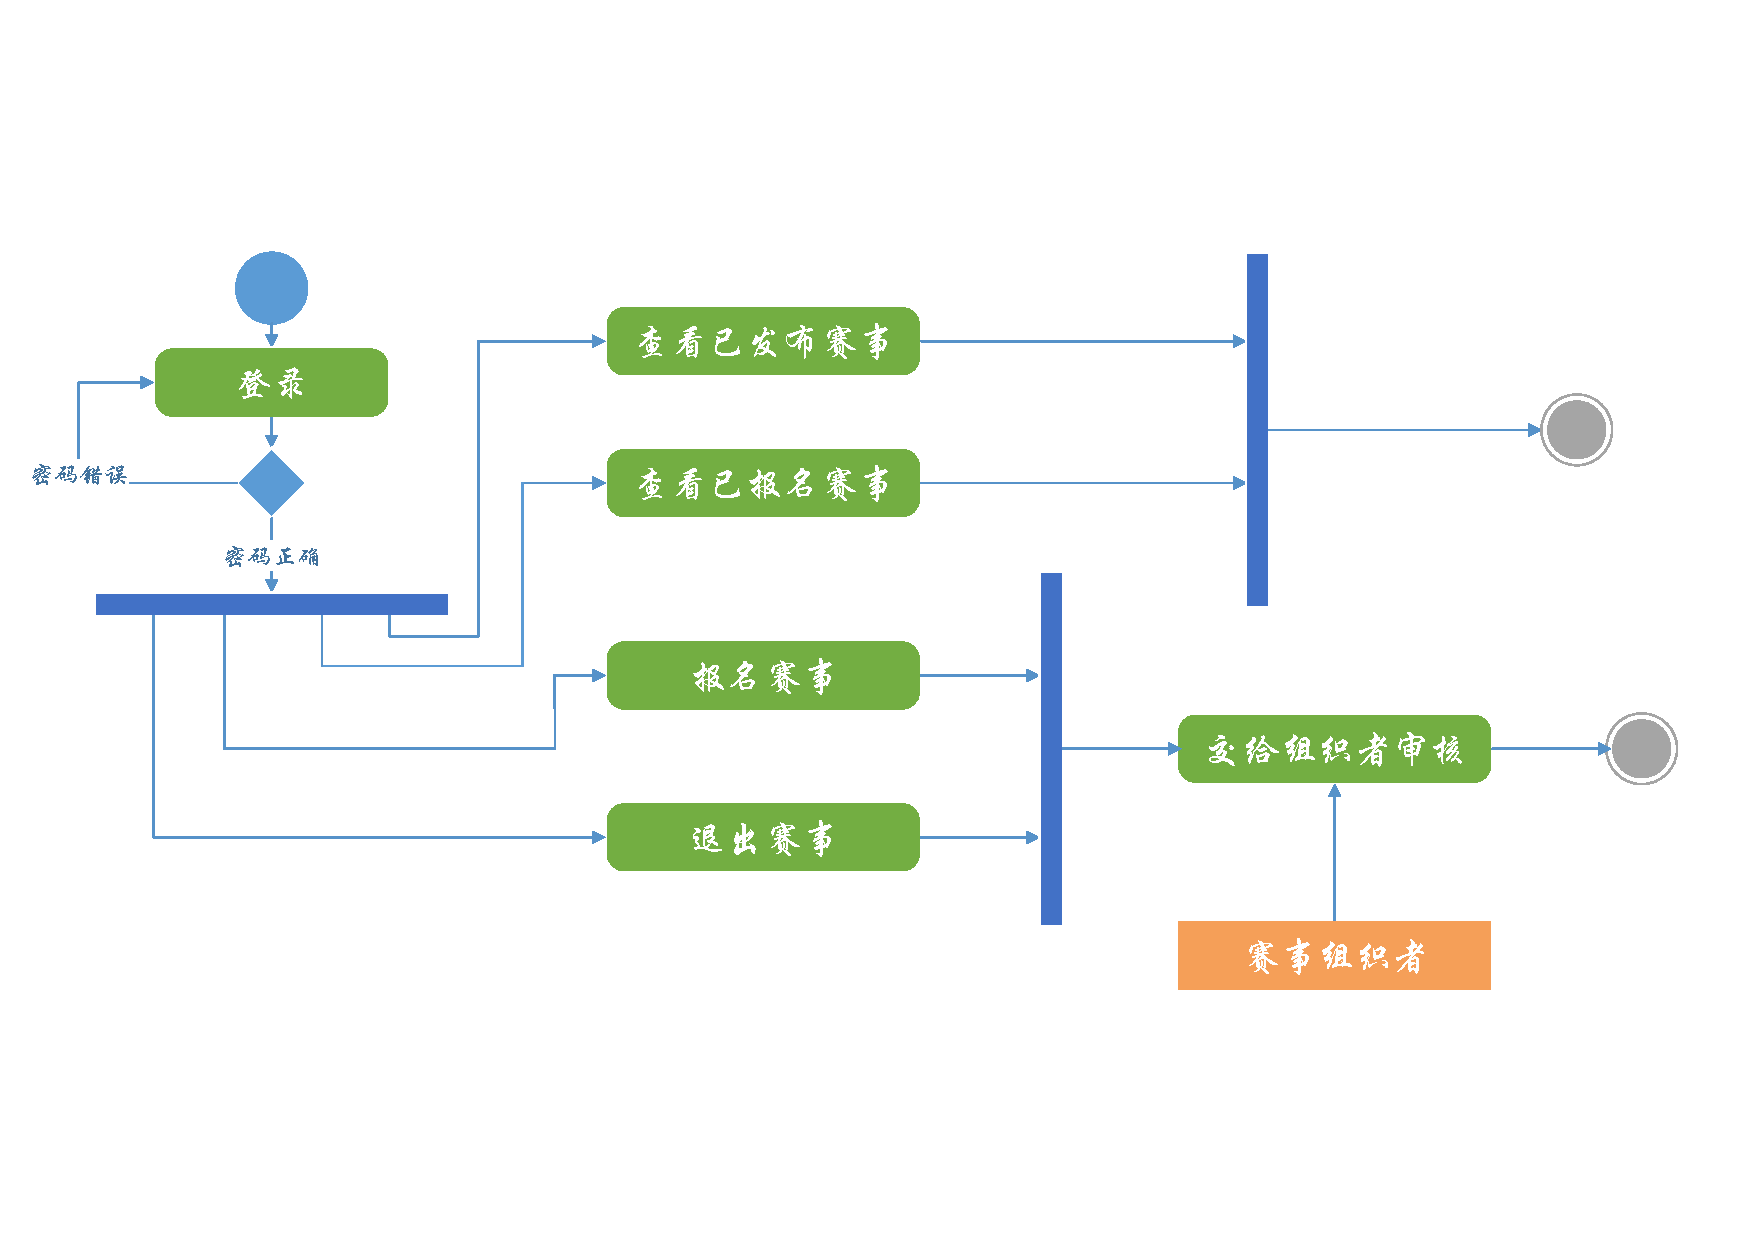
\includegraphics[width=1\columnwidth]{ac1}
	
}

\subsubsection{赛事组织者用户活动图}
{\centering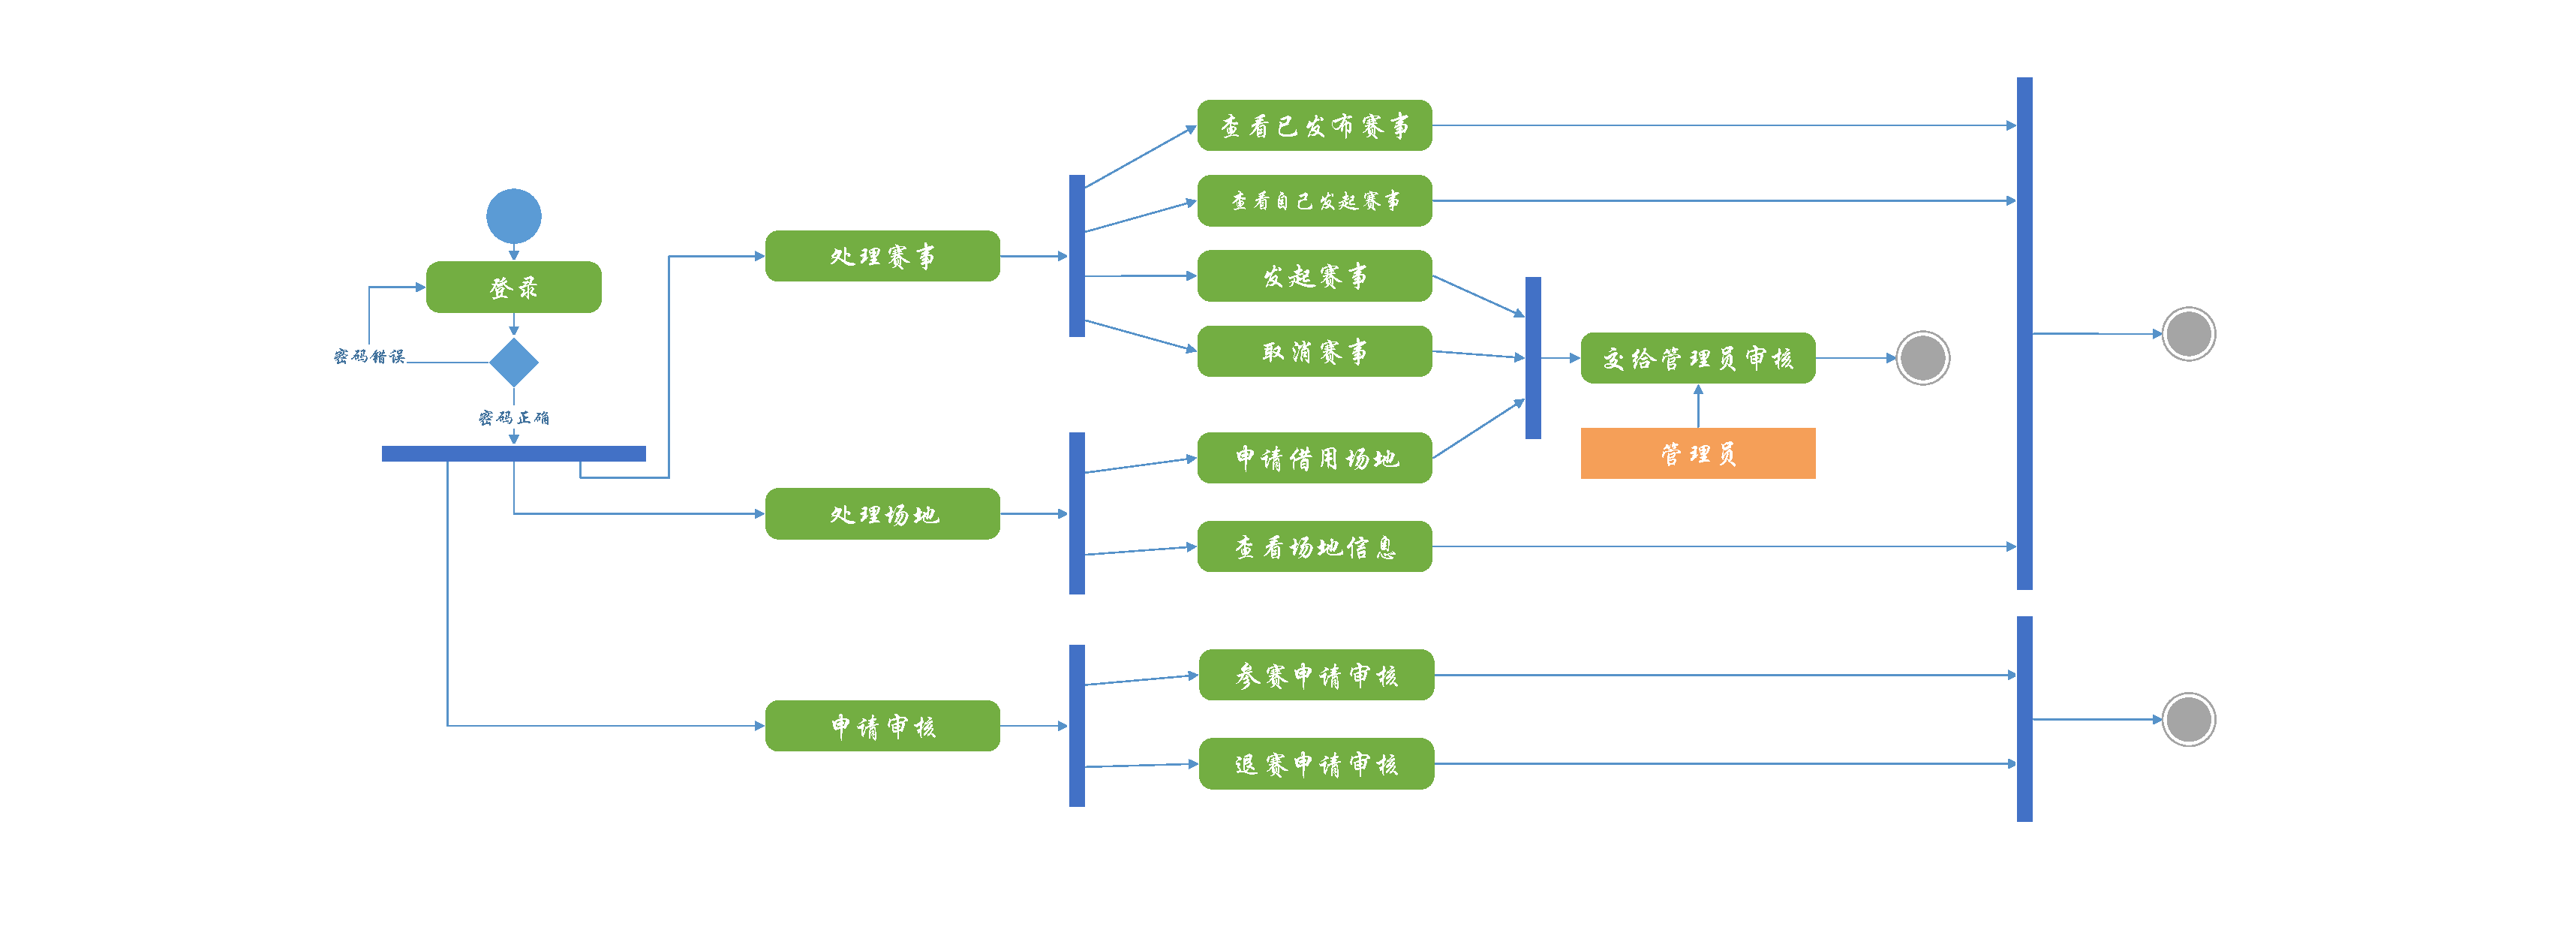
\includegraphics[width=1\columnwidth]{ac2}
	
}

\subsubsection{管理员用户活动图}
{\centering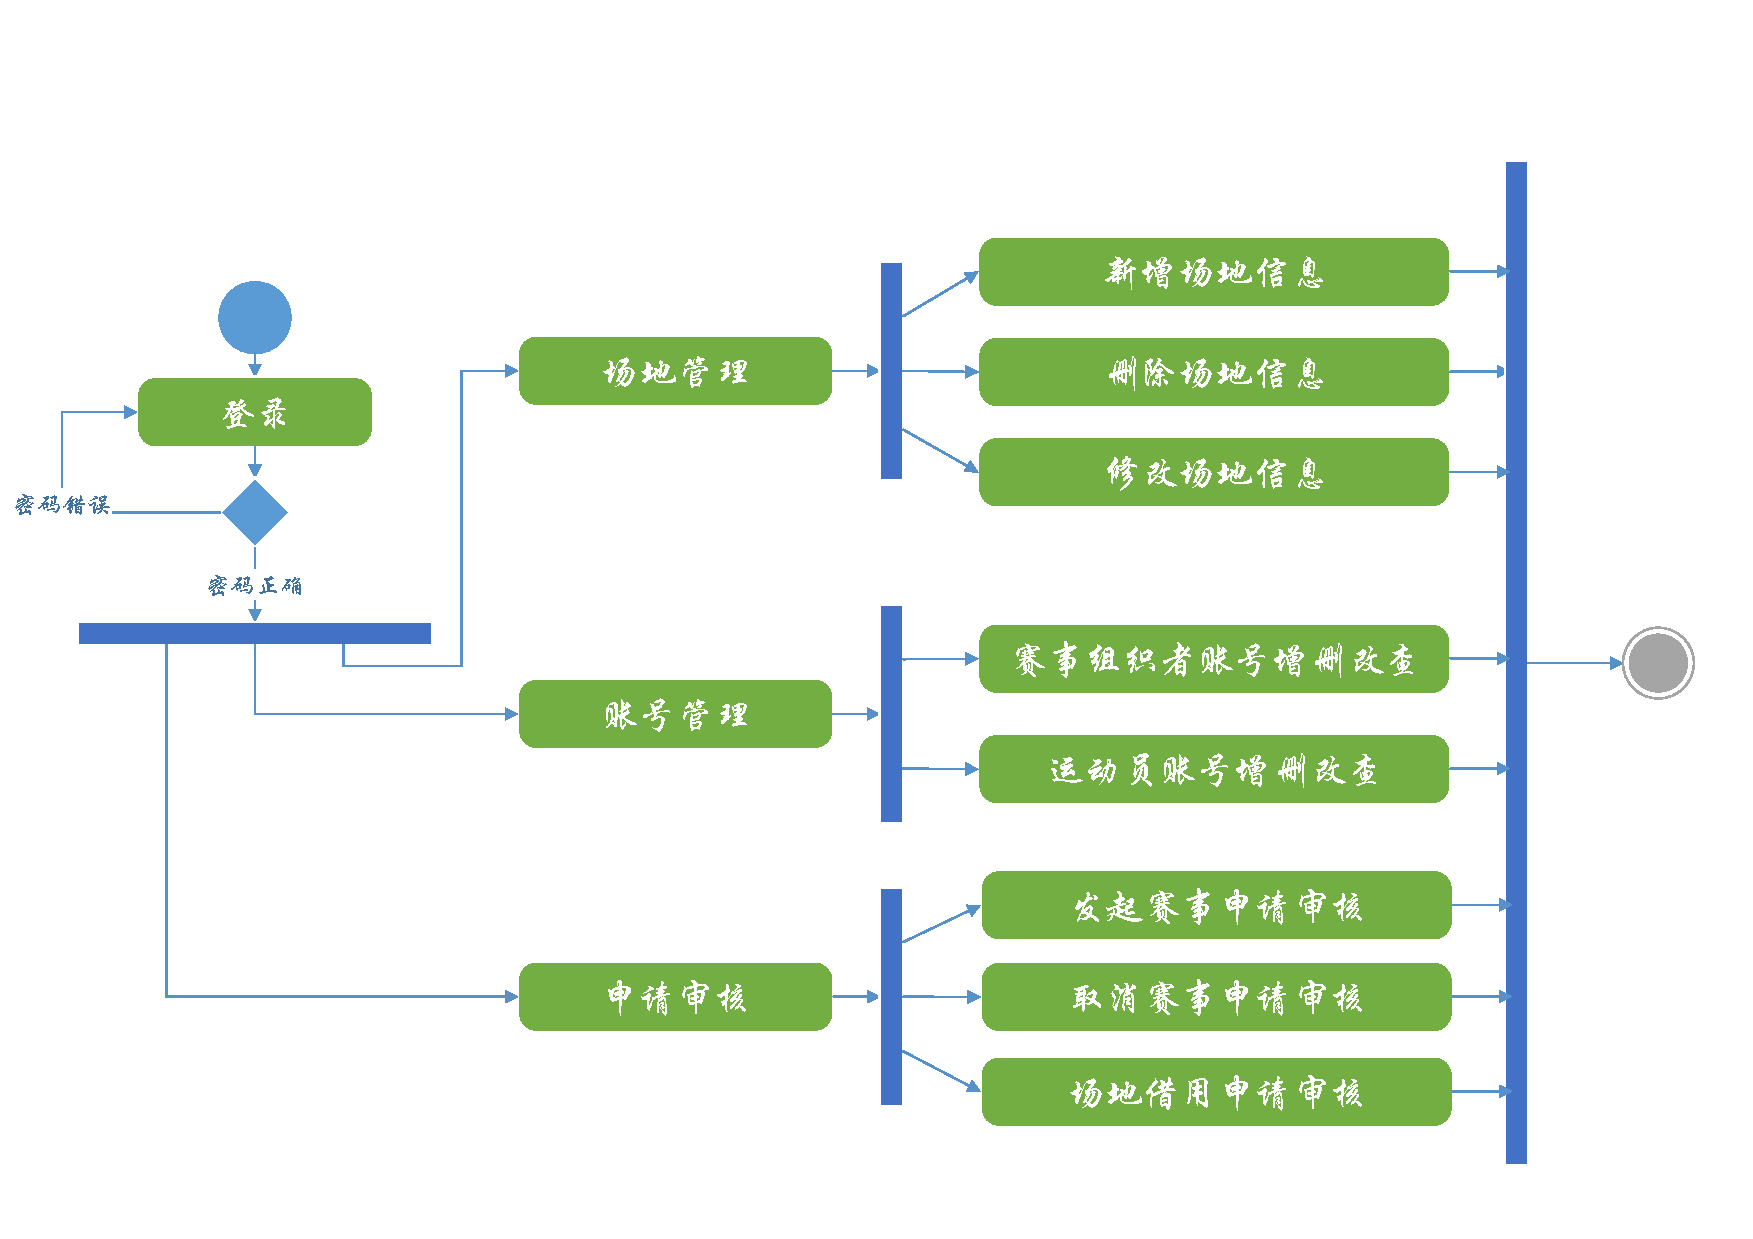
\includegraphics[width=1\columnwidth]{ac3}
	
}


\subsection{数据模型}
{\centering\includegraphics[width=1\columnwidth]{ER}
	
}


\section{软件设计}
\subsection{软件体系结构设计}
{\centering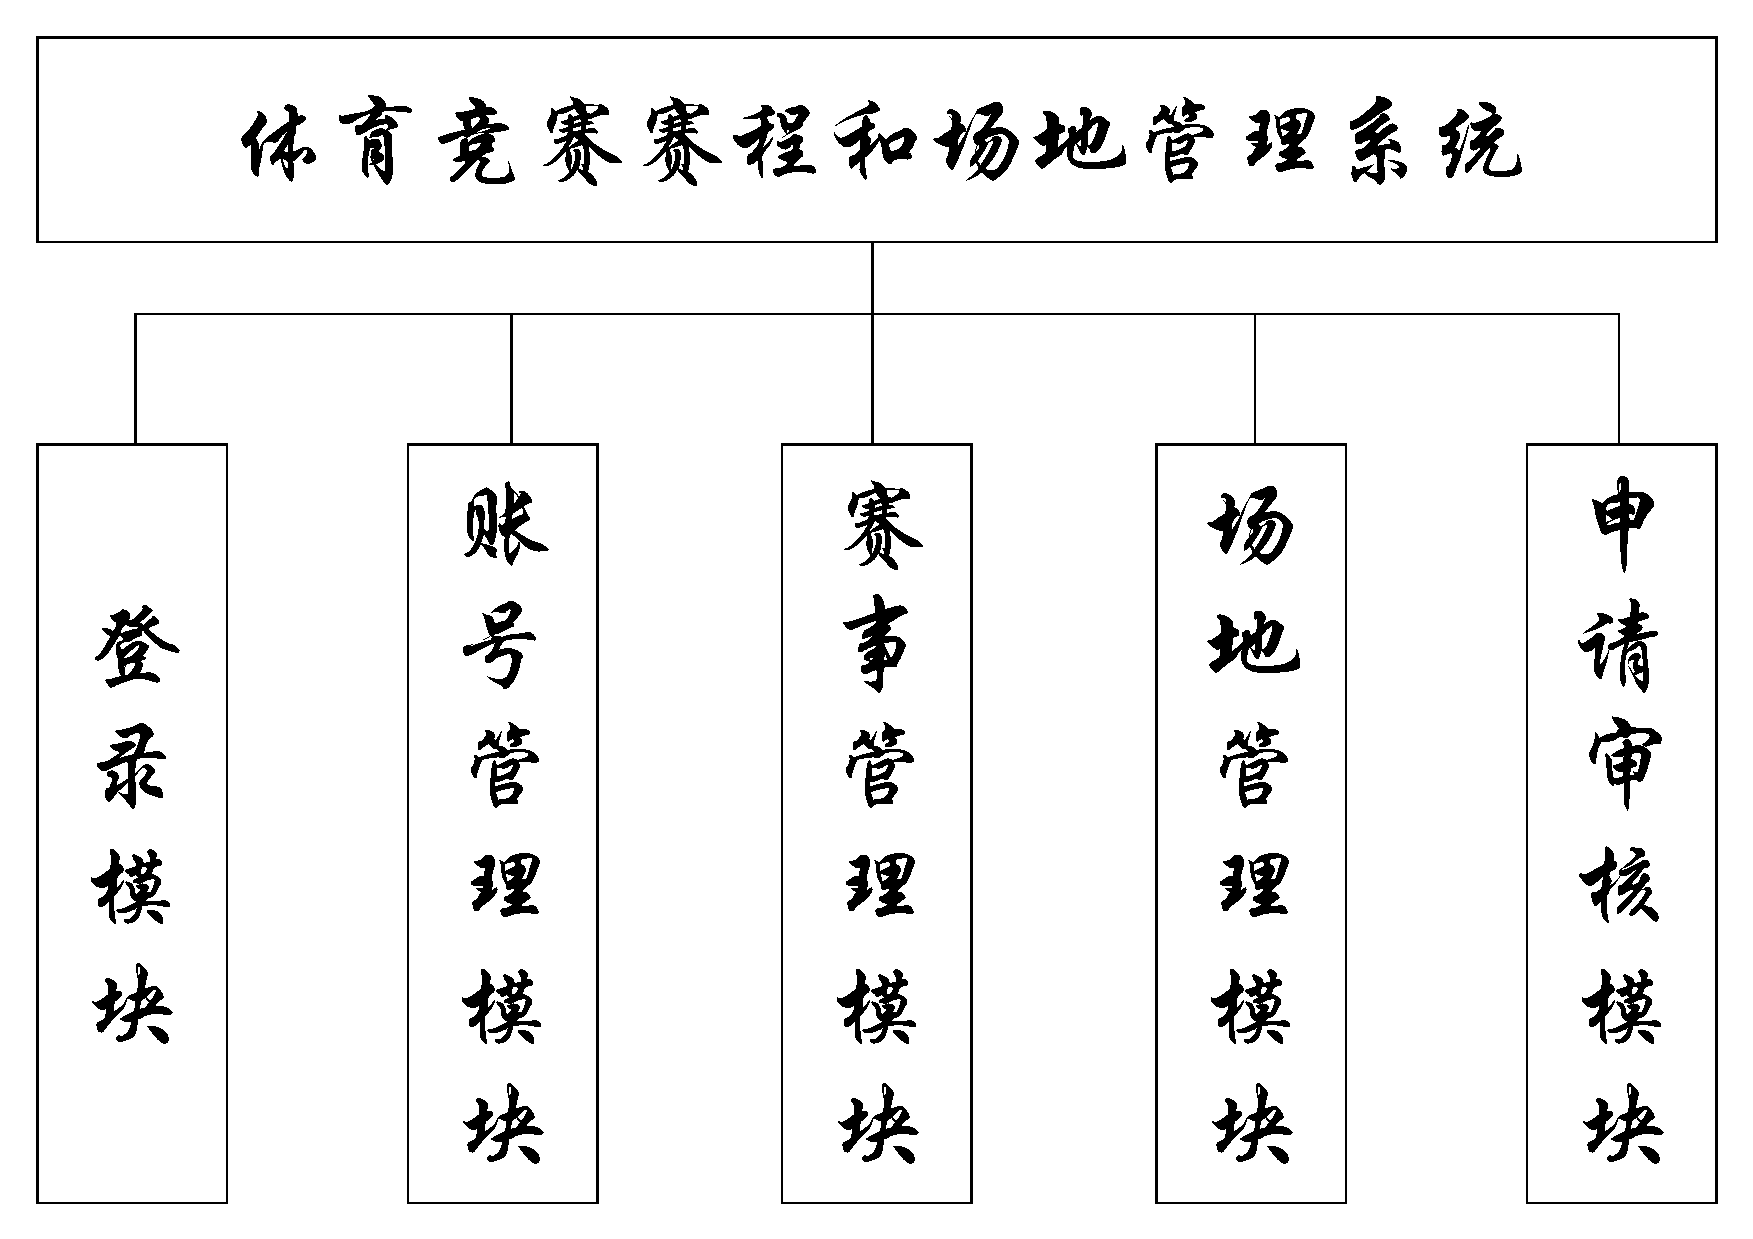
\includegraphics[width=1\columnwidth]{1}
	
}

如图所示,体育竞赛赛程和场地管理系统总共由五个模块构成,包括登录模块、账号管理模块、赛事管理模块、场地管理模块和申请审核模块。

其中,登录模块包含用户登陆界面、帐号密码校验、引导初次登录的赛事组织者与运动员用户修改初始密码并完善个人信息等功能;账号管理模块包含对赛事组织者与运动员用户账号的新增、删除、修改与查看功能;赛事管理模块包含已发布赛事查看、已报名赛事查看、赛事报名、赛事退出、已发布赛事查看、自己发起赛事的查看、赛事发起、赛事取消等功能;场地管理模块包含场地信息新增、场地信息删除、场地信息修改、场地信息查看、场地借用申请等功能;申请审核模块包含参赛申请审核、退赛申请审核、发起赛事申请审核、取消赛事申请审核、场地借用申请审核等功能。

各模块可以独立进行开发。由于系统严格控制权限访问,用户在经过身份认证后,只能使用其权限等级所对应的部分功能,访问其权限范围内的数据,进行其权限范围内的操作。


\subsection{类的设计}
{\centering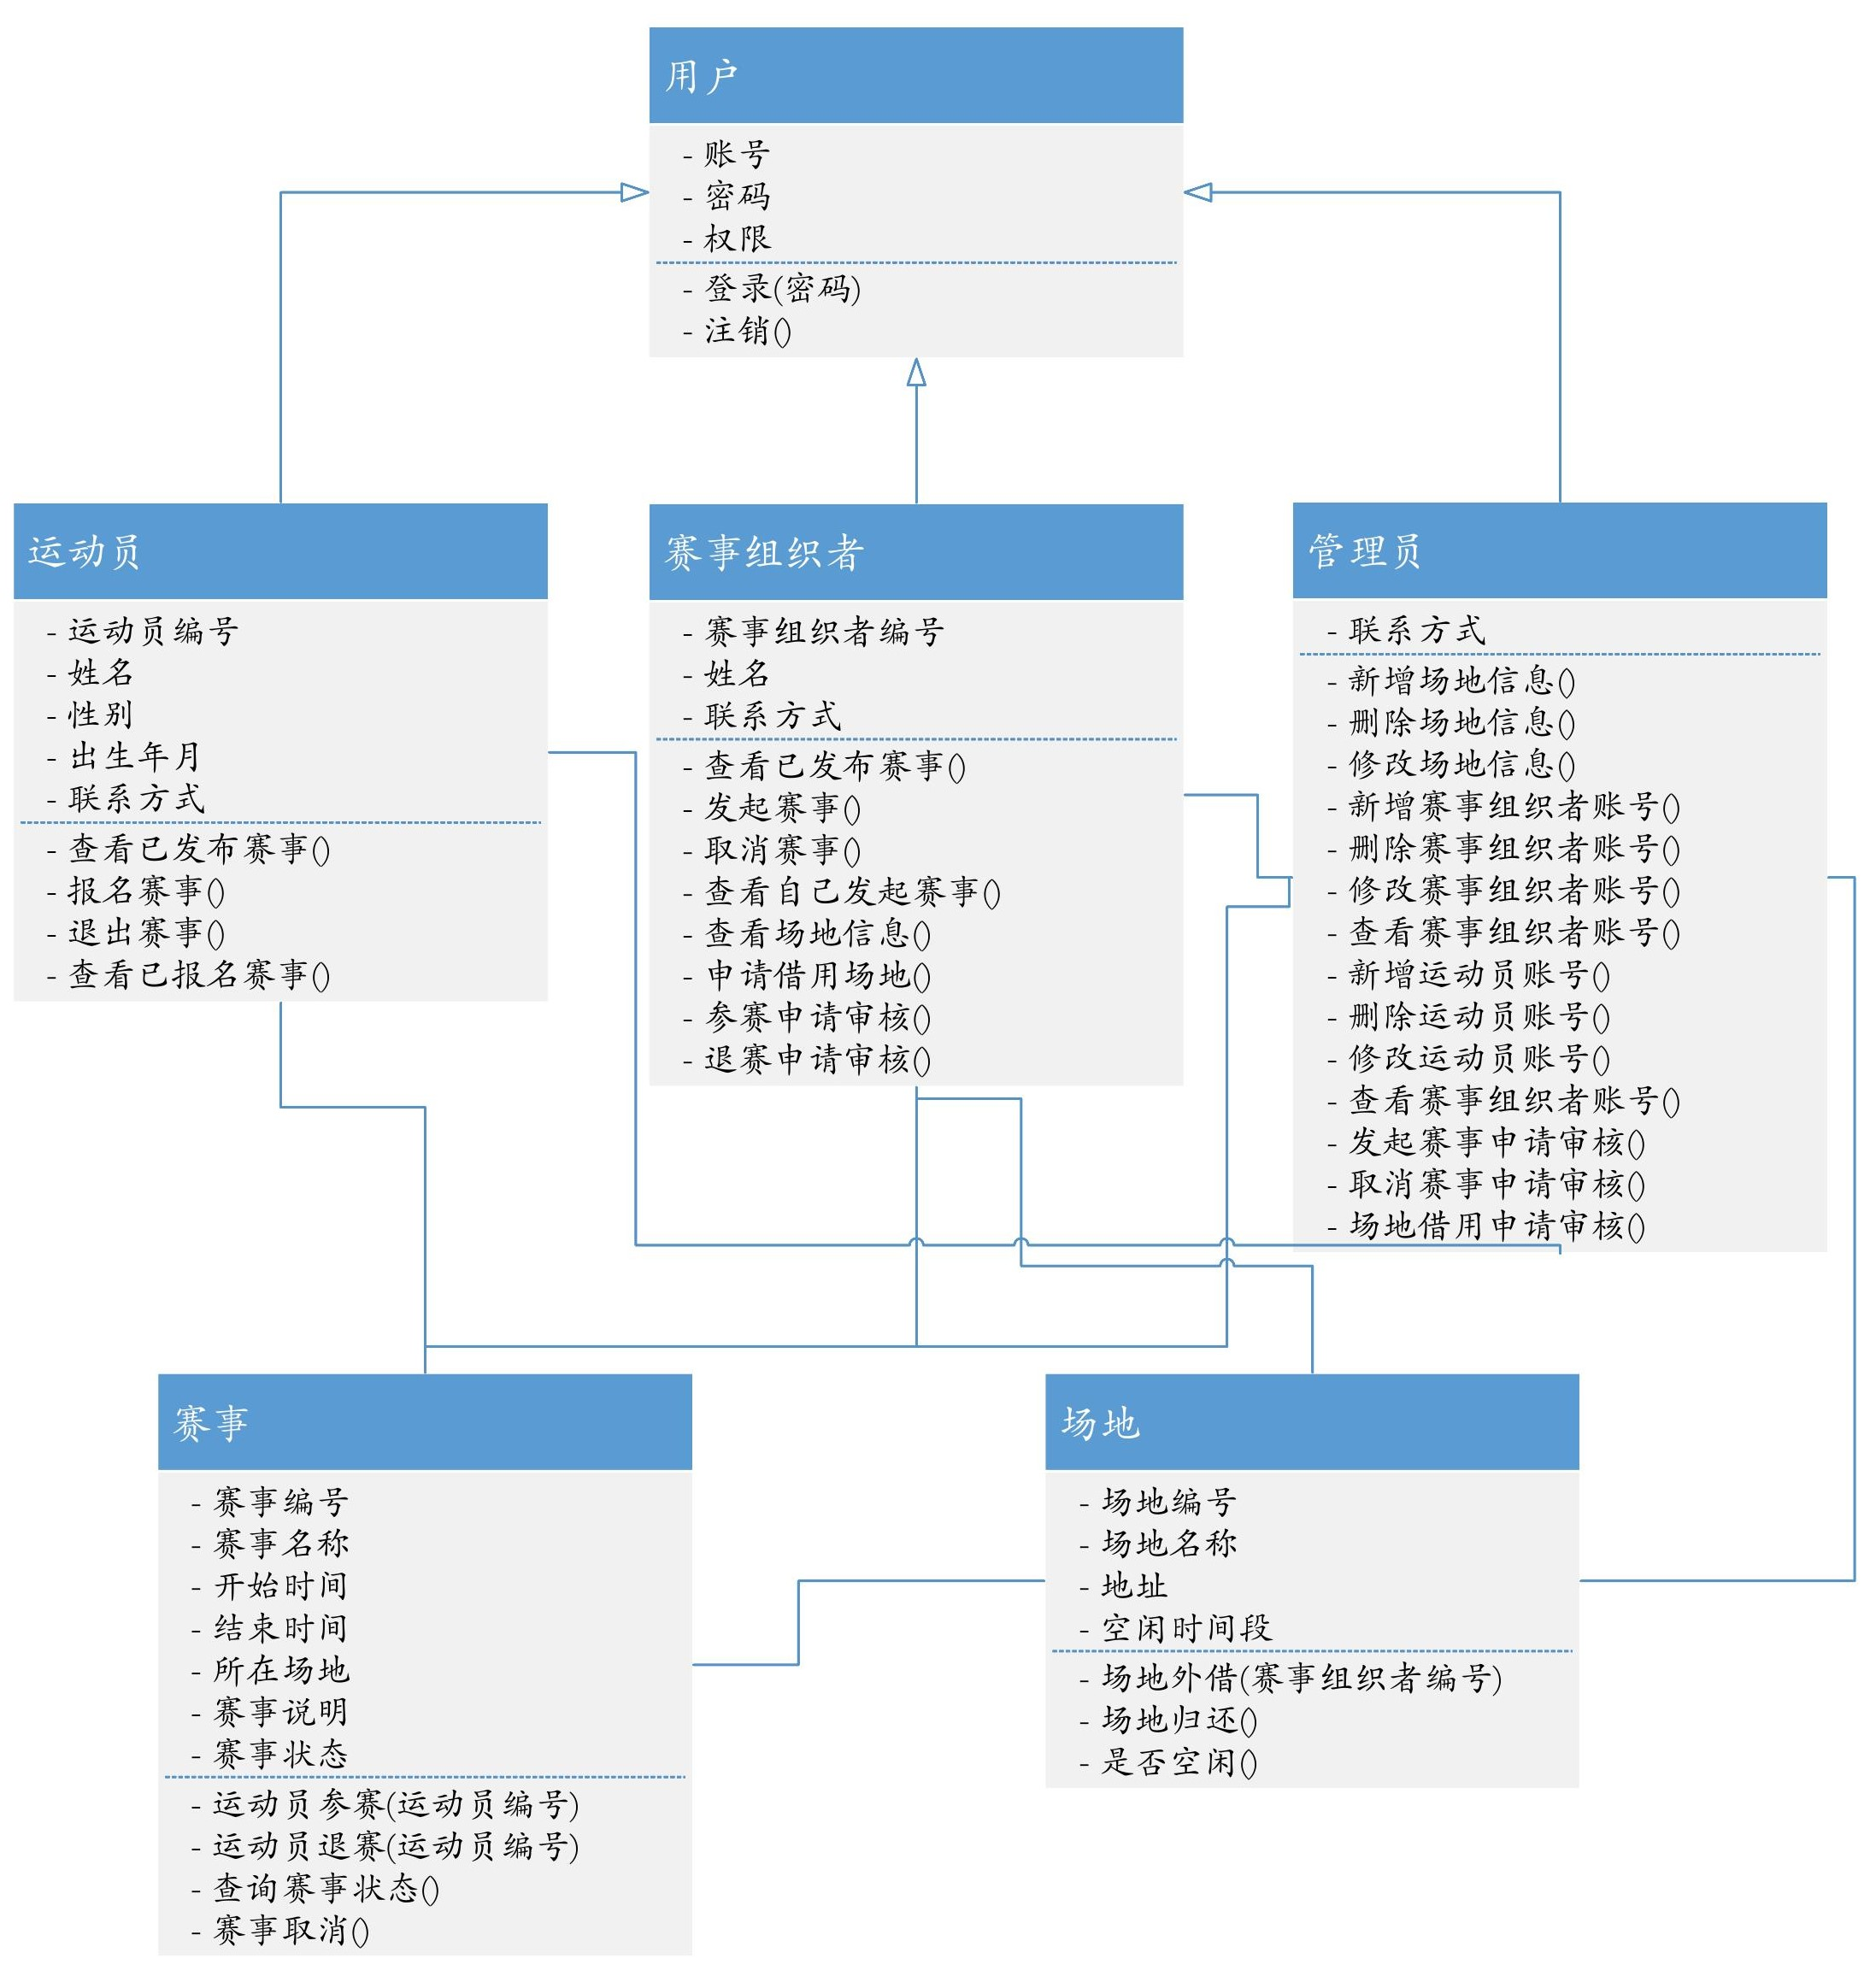
\includegraphics[width=1\columnwidth]{class.jpg}
	
}

\subsection{交互模型}

\paragraph{运动员用户赛事报名时序图}
{\centering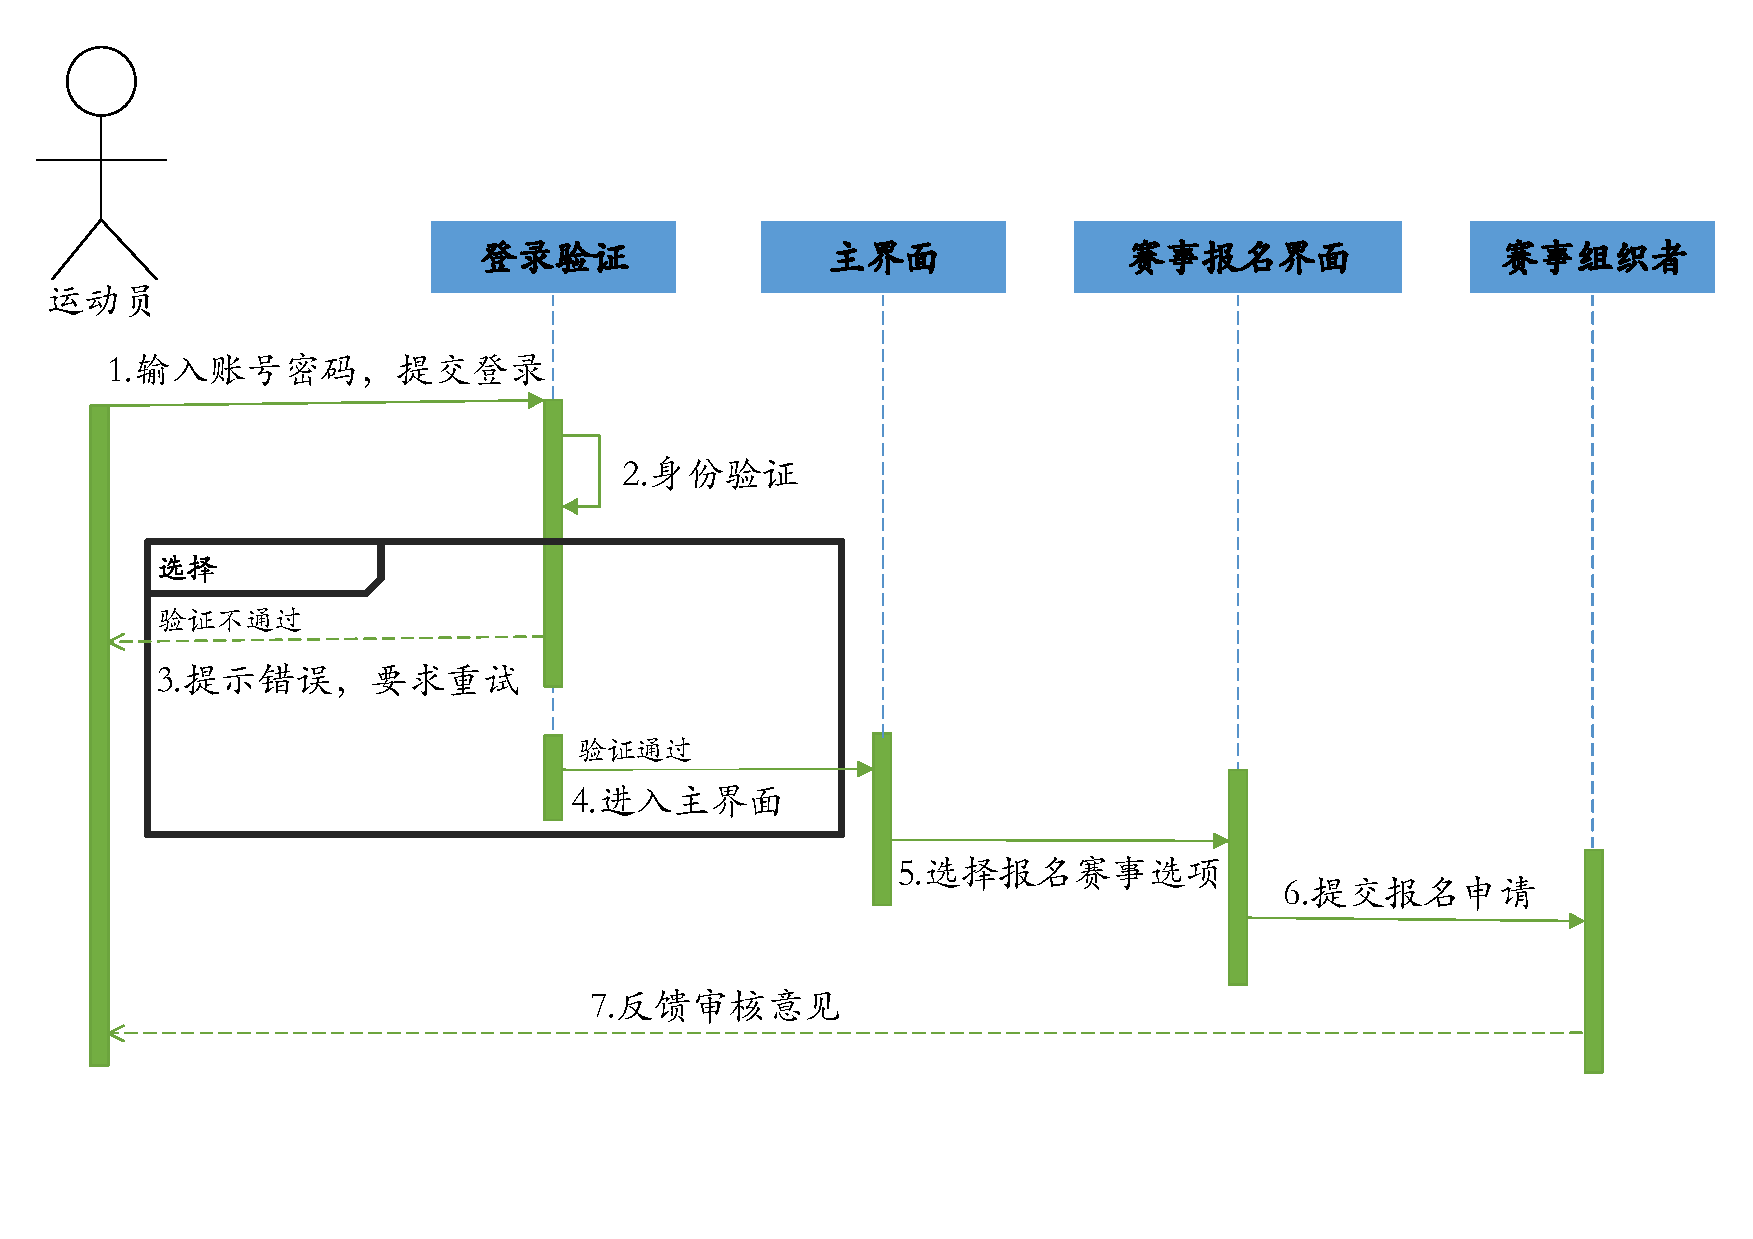
\includegraphics[width=1\columnwidth]{sd1}
	
}

\paragraph{赛事组织者用户赛事发起时序图}
{\centering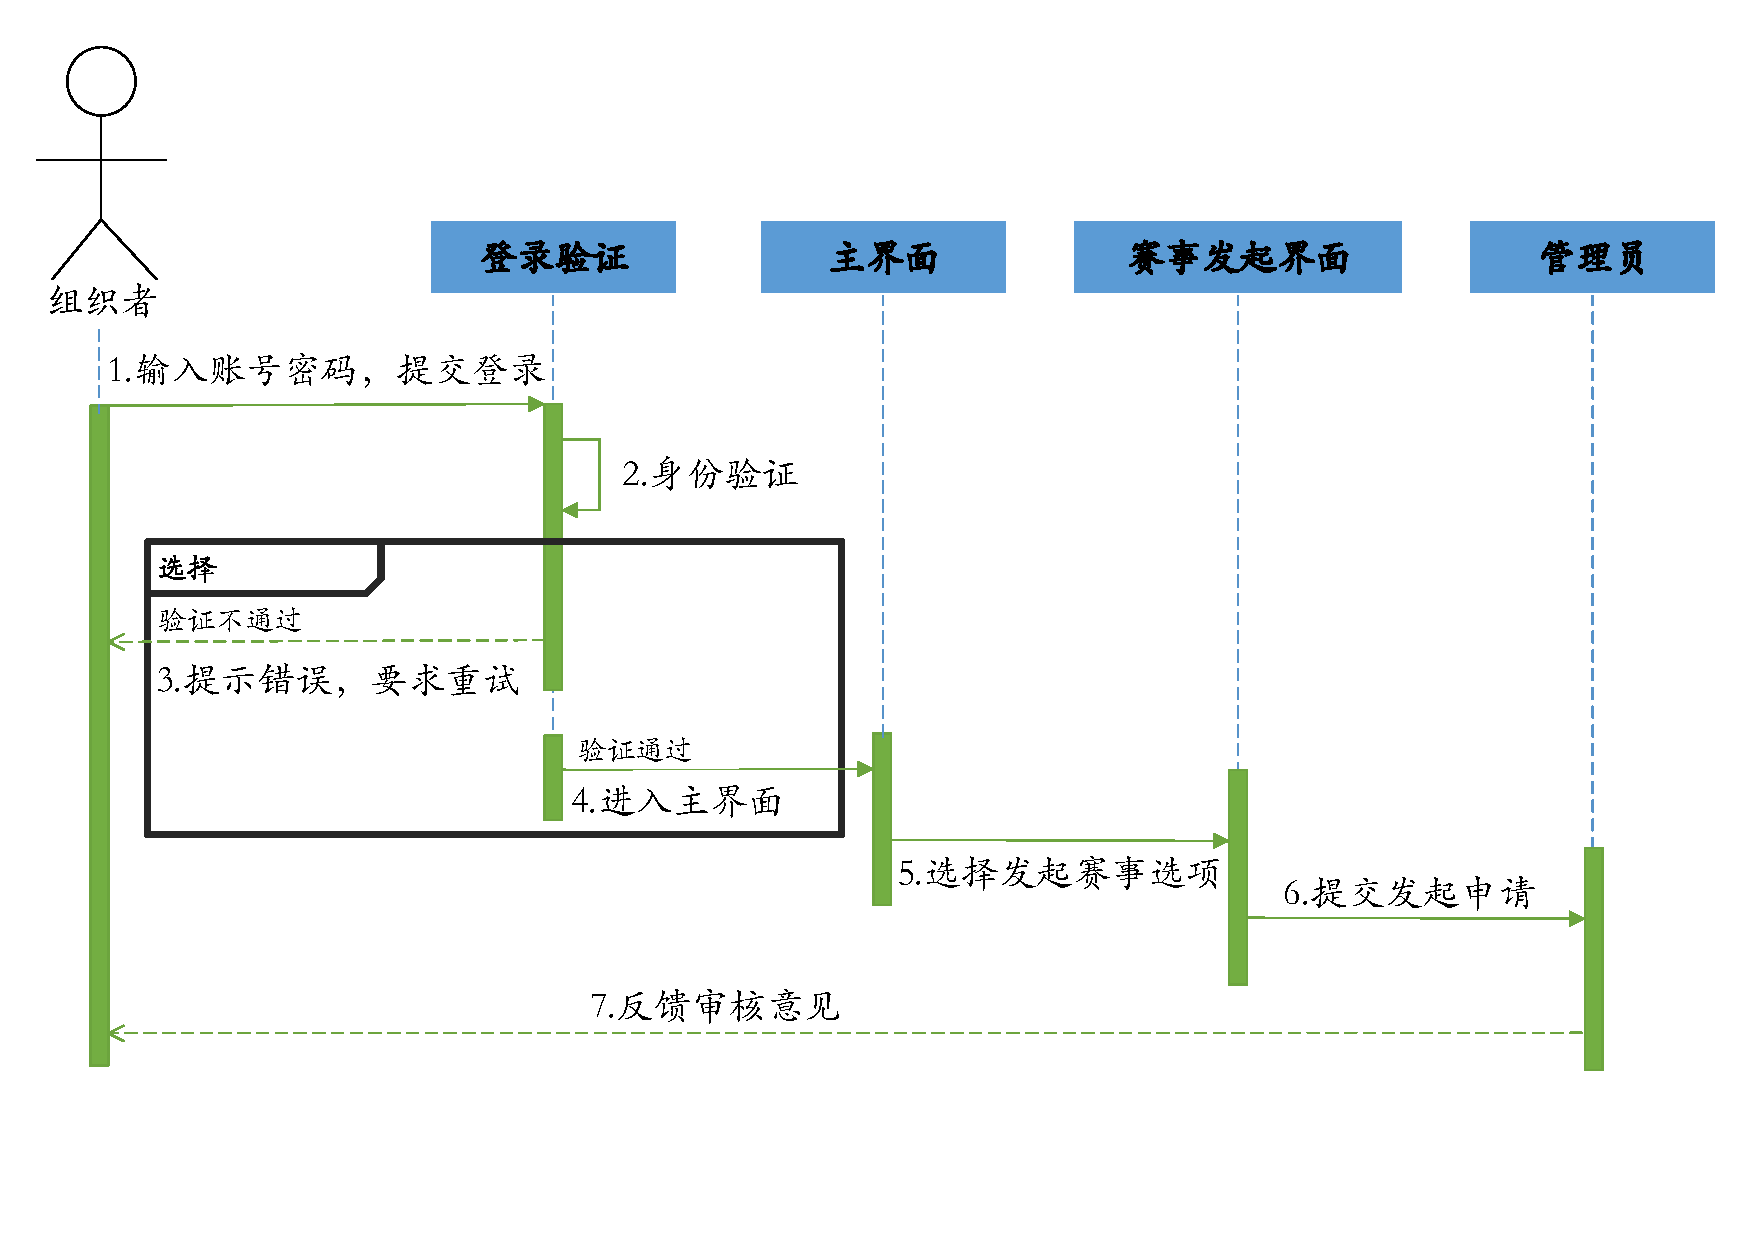
\includegraphics[width=1\columnwidth]{sd2}
	
}

%\paragraph{运动员用户赛事报名时序图}
%{\centering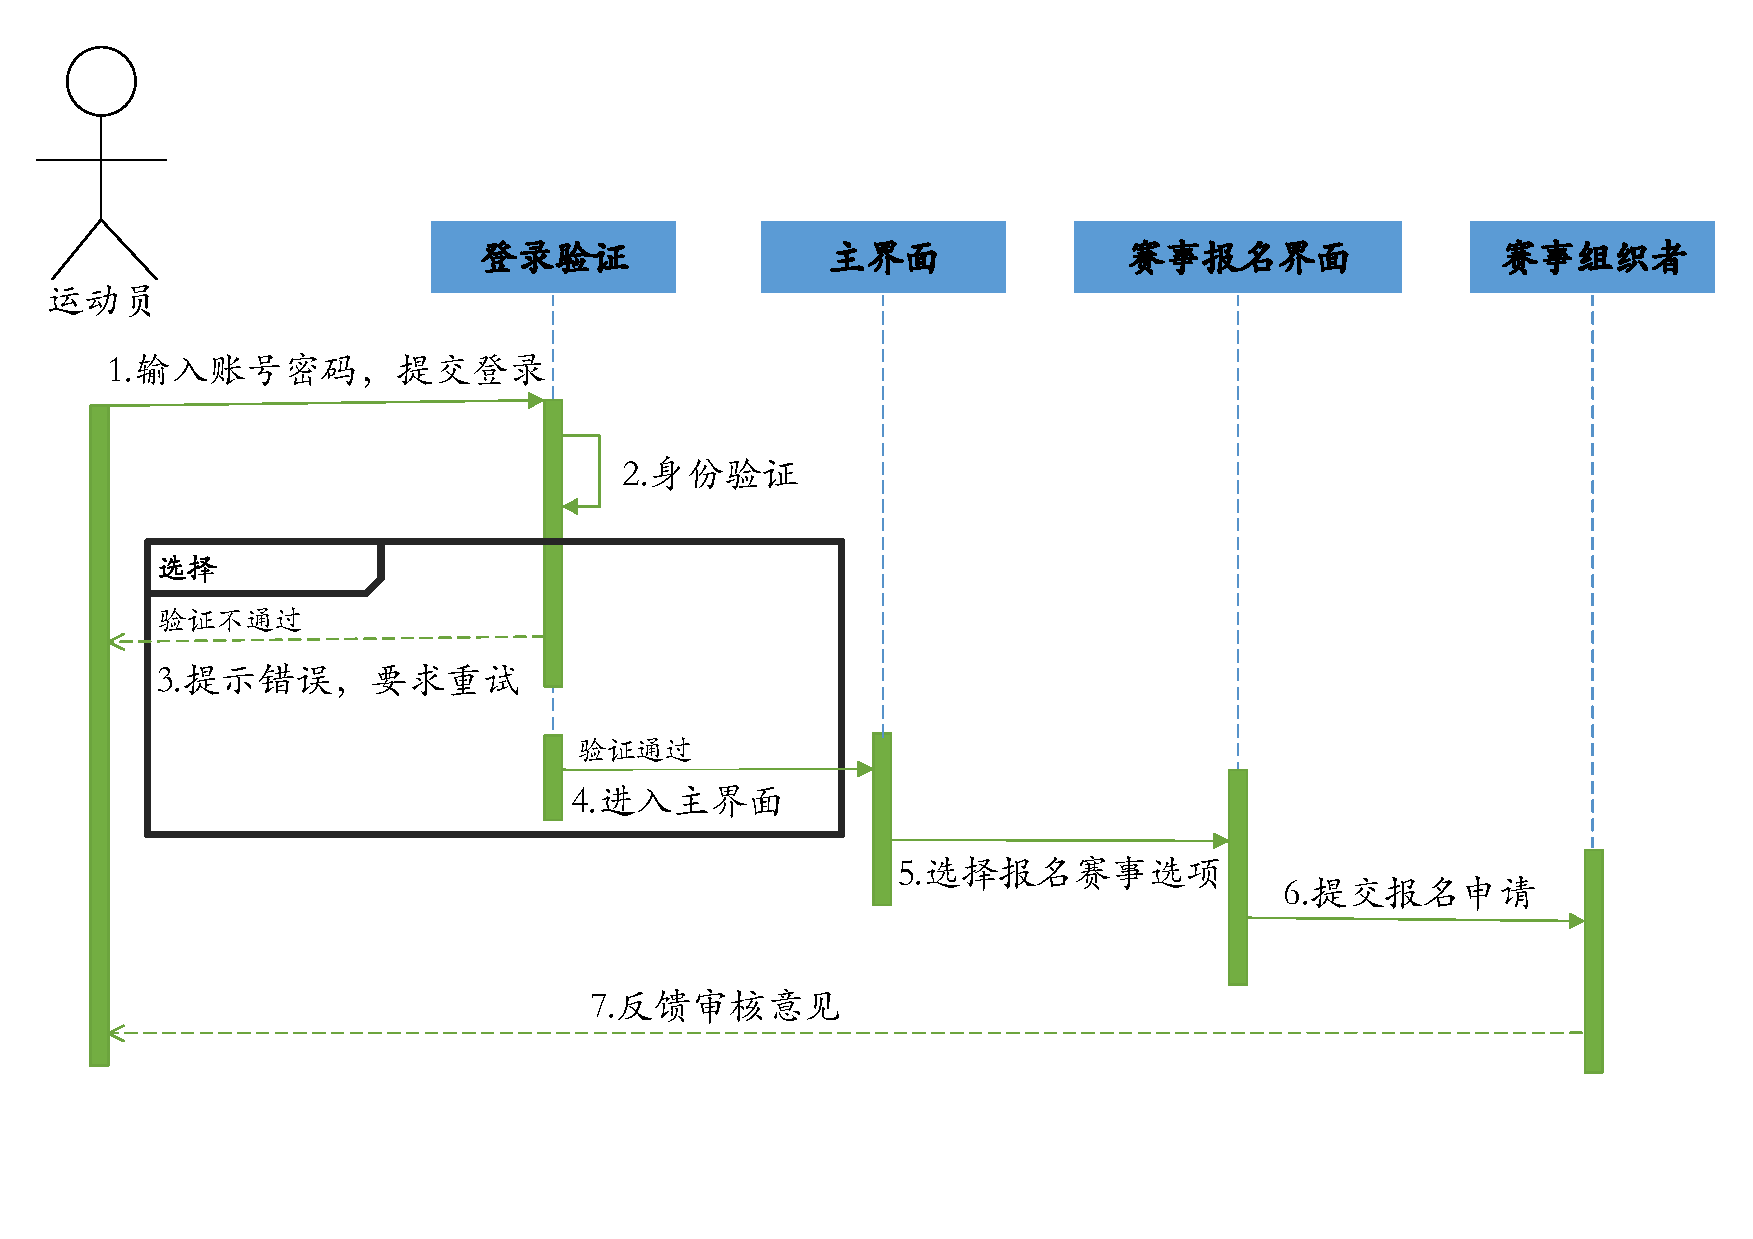
\includegraphics[width=1\columnwidth]{sd1}
	
%}

%\paragraph{运动员用户赛事报名时序图}
%{\centering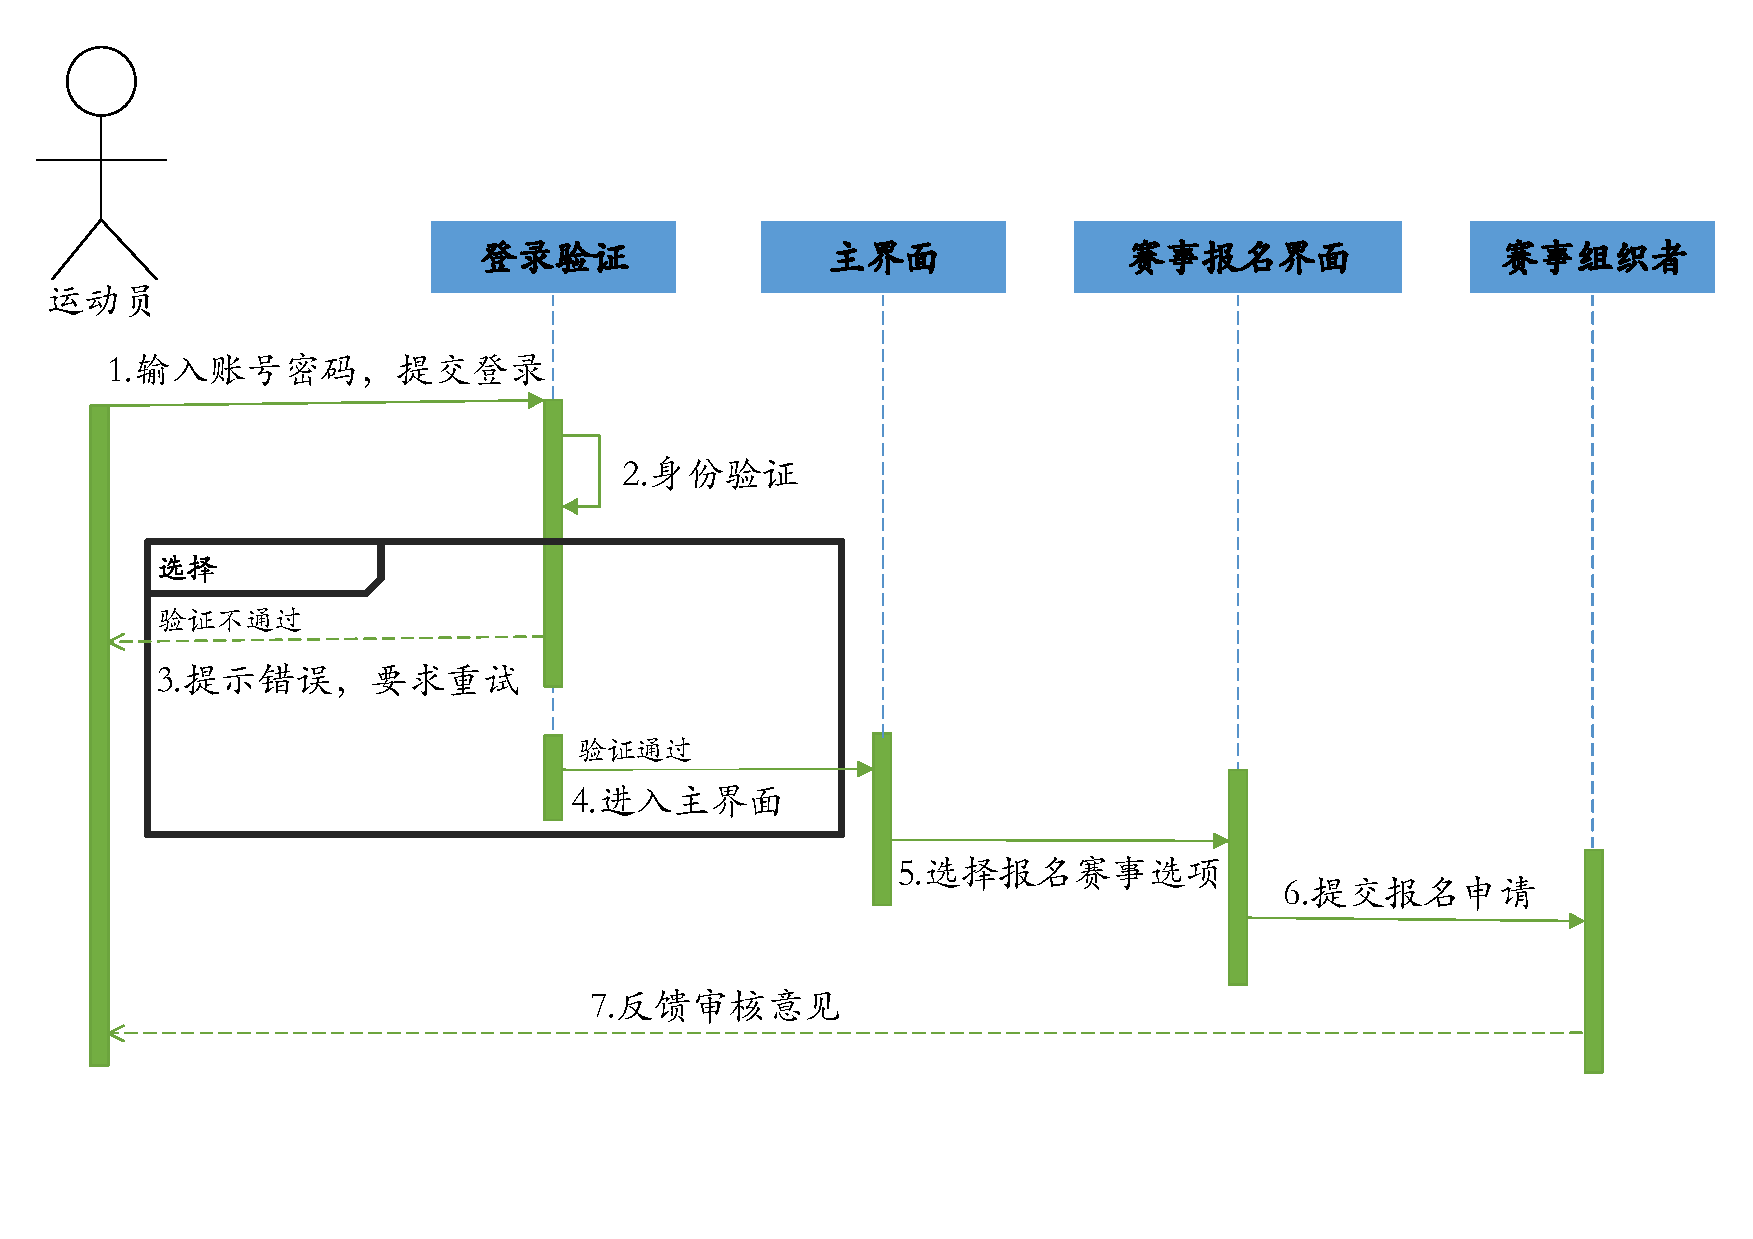
\includegraphics[width=1\columnwidth]{sd1}
	
%}

\subsection{数据库设计}
\subsubsection{ER图}
{\centering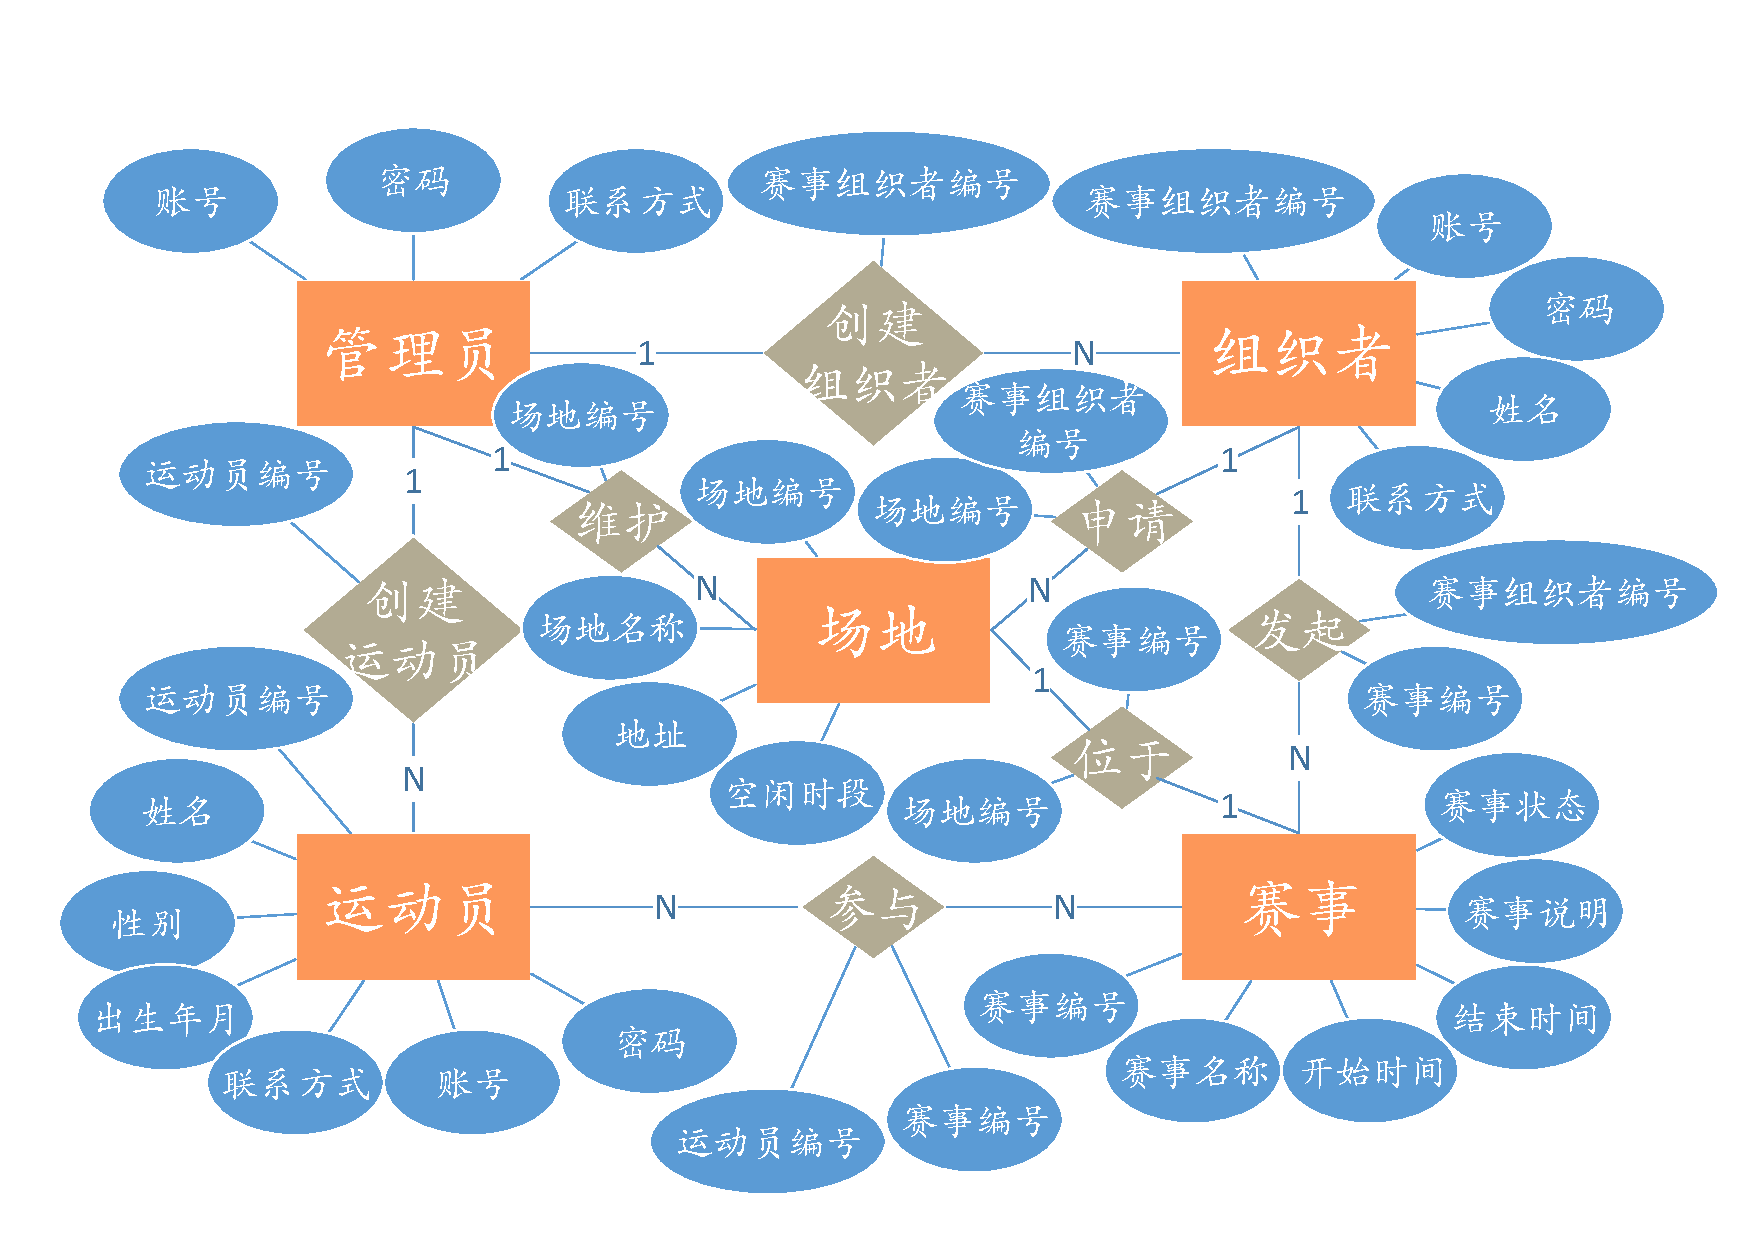
\includegraphics[width=1\columnwidth]{er}
	
}

\subsubsection{表结构}
\begin{table}[H]
	\centering
	\caption{Athlete(运动员)}
	\label{table:Tab_db_athlete}
	\begin{tabular}{|c|c|c|c|c|c|c|}
		\hline\noalign{\smallskip}
		AthleteID & Account & Password & Name & Gender & Birthday & Tel\\
		\hline
		varchar2(7) & varchar2(9) & varchar2(16) & varchar2(20) & varchar2(12) & date & varchar2(11)\\
		\noalign{\smallskip}
		\hline
		\noalign{\smallskip}
	\end{tabular}

	\caption{Organizer(赛事组织者)}
	\label{table:Tab_db_organizer}
	\begin{tabular}{|c|c|c|c|c|}
		\hline\noalign{\smallskip}
		OrganizerID & Account & Password & Name & Tel\\
		\hline
		varchar2(7) & varchar2(9) & varchar2(16) & varchar2(20) & varchar2(11)\\
		\noalign{\smallskip}
		\hline
		\noalign{\smallskip}
	\end{tabular}

	\caption{Admin(管理员)}
	\label{table:Tab_db_admin}
	\begin{tabular}{|c|c|c|}
		\hline\noalign{\smallskip}
		Account & Password & Tel\\
		\hline
		varchar2(5) & varchar2(16) & varchar2(11)\\
		\noalign{\smallskip}
		\hline
		\noalign{\smallskip}
	\end{tabular}

	\caption{Event(赛事)}
	\label{table:Tab_db_event}
	\begin{tabular}{|c|c|c|c|c|c|}
		\hline\noalign{\smallskip}
		EventID & Name & StartTime & EndTime & Status & Description\\
		\hline
		varchar2(7) & varchar2(40) & date & date & varchar2(10) & varchar2(100)\\
		\noalign{\smallskip}
		\hline
		\noalign{\smallskip}
	\end{tabular}
\end{table}

\begin{table}[H]
	\centering
	\caption{Site(场地)}
	\label{table:Tab_db_site}
	\begin{tabular}{|c|c|c|c|}
		\hline\noalign{\smallskip}
		SiteID & Name & LeisureTime & Address \\
		\hline
		varchar2(7) & varchar2(40) & varchar2(100) & varchar2(100)\\
		\noalign{\smallskip}
		\hline
		\noalign{\smallskip}
	\end{tabular}

	\caption{CreateAthlete(创建运动员}
	\label{table:Tab_db_ca}
	\begin{tabular}{|c|}
		\hline\noalign{\smallskip}
		AthleteID  \\
		\hline
		varchar2(7) \\
		\noalign{\smallskip}
		\hline
		\noalign{\smallskip}
	\end{tabular}
		
	\caption{CreateOrganizer(创建组织者)}
	\label{table:Tab_db_co}
	\begin{tabular}{|c|}
		\hline\noalign{\smallskip}
		OrganizerID  \\
		\hline
		varchar2(7) \\
		\noalign{\smallskip}
		\hline
		\noalign{\smallskip}
	\end{tabular}

	\caption{Maintain(维护)}
	\label{table:Tab_db_maintain}
	\begin{tabular}{|c|}
		\hline\noalign{\smallskip}
		SiteID \\
		\hline
		varchar2(7) \\
		\noalign{\smallskip}
		\hline
		\noalign{\smallskip}
	\end{tabular}
	
	\caption{Apply(申请)}
	\label{table:Tab_db_apply}
	\begin{tabular}{|c|c|}
		\hline\noalign{\smallskip}
		SiteID & OrganizerID \\
		\hline
		varchar2(7) & varchar2(7) \\
		\noalign{\smallskip}
		\hline
		\noalign{\smallskip}
	\end{tabular}

	\caption{Launch(发起)}
	\label{table:Tab_db_launch}
	\begin{tabular}{|c|c|}
		\hline\noalign{\smallskip}
		EventID & OrganizerID \\
		\hline
		varchar2(7) & varchar2(7) \\
		\noalign{\smallskip}
		\hline
		\noalign{\smallskip}
	\end{tabular}

	\caption{At(位于)}
	\label{table:Tab_db_at}
	\begin{tabular}{|c|c|}
		\hline\noalign{\smallskip}
		EventID & SiteID \\
		\hline
		varchar2(7) & varchar2(7) \\
		\noalign{\smallskip}
		\hline
		\noalign{\smallskip}
	\end{tabular}

	\caption{Participate(参与)}
	\label{table:Tab_db_participate}
	\begin{tabular}{|c|c|}
		\hline\noalign{\smallskip}
		AthleteID & EventID \\
		\hline
		varchar2(7) & varchar2(7) \\
		\noalign{\smallskip}
		\hline
		\noalign{\smallskip}
	\end{tabular}
\end{table}


\section{程序运行结果}
本节演示一些程序功能及相应运行结果。

{\centering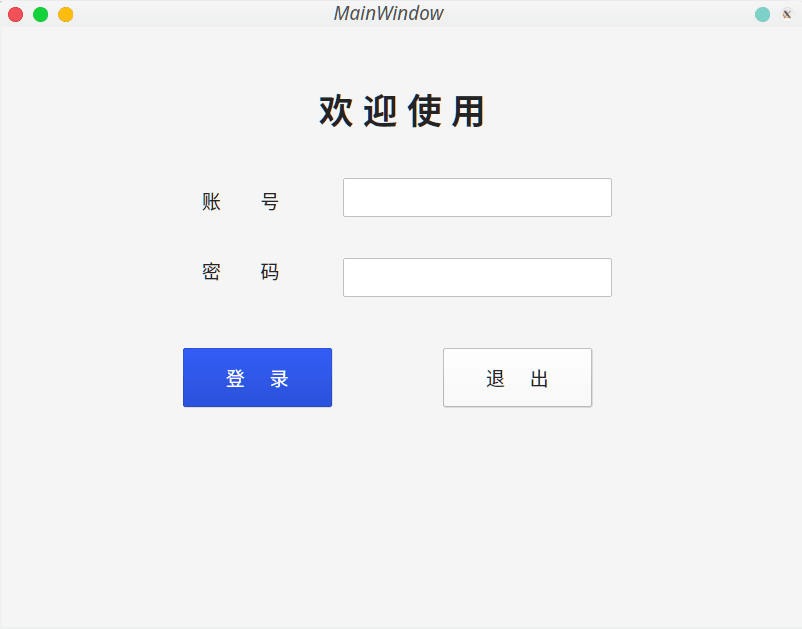
\includegraphics[width=1\columnwidth]{1.png}
	
}

系统启动后进入登录界面,显示“欢迎使用”字样,并提供账号和密码的文本输入框。完成输入后用户可通过按下“登录”按钮进行身份验证以登录系统。在提交登录前,用户可随时按下“退出”按钮退出本系统。

{\centering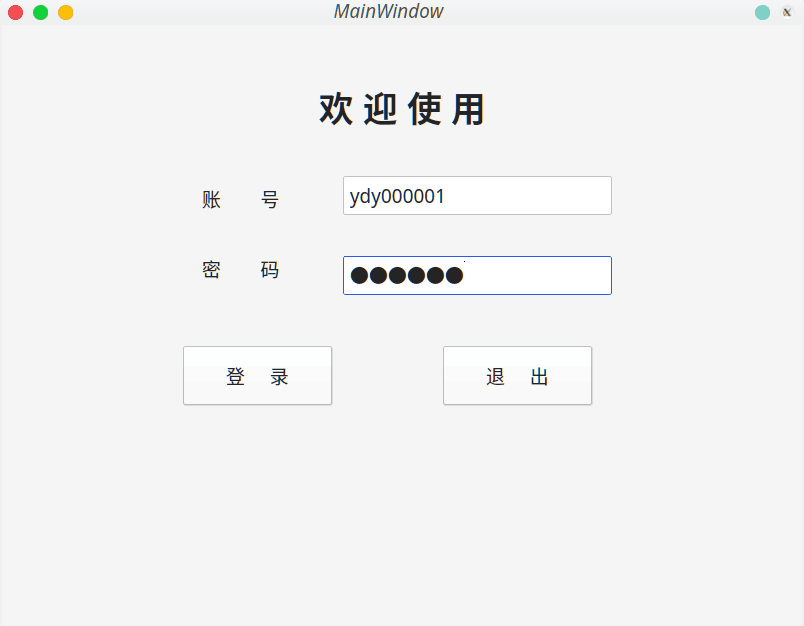
\includegraphics[width=1\columnwidth]{2.png}
	
}

输入的密码内容被加密显示,以保护用户个人账号安全。

{\centering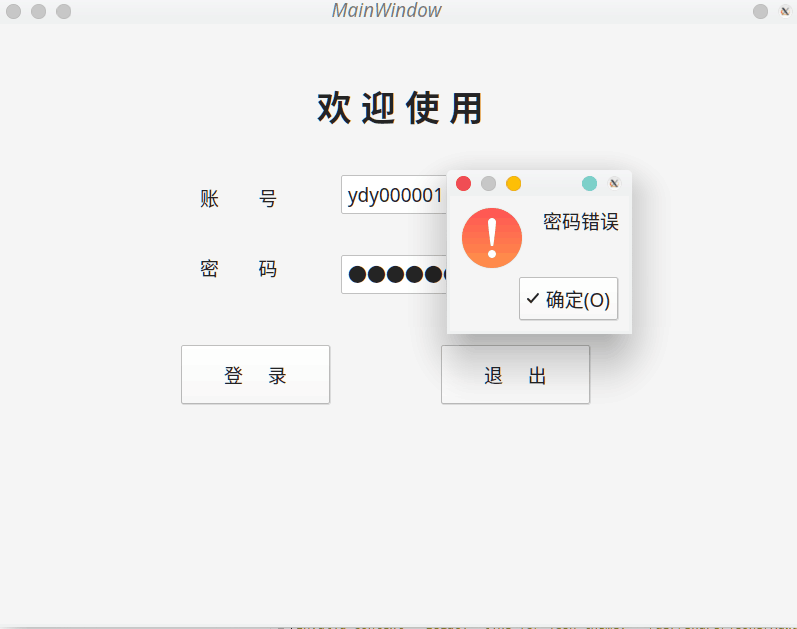
\includegraphics[width=1\columnwidth]{3.png}
	
}

当用户输入的密码错误时,系统提示“密码错误”。

{\centering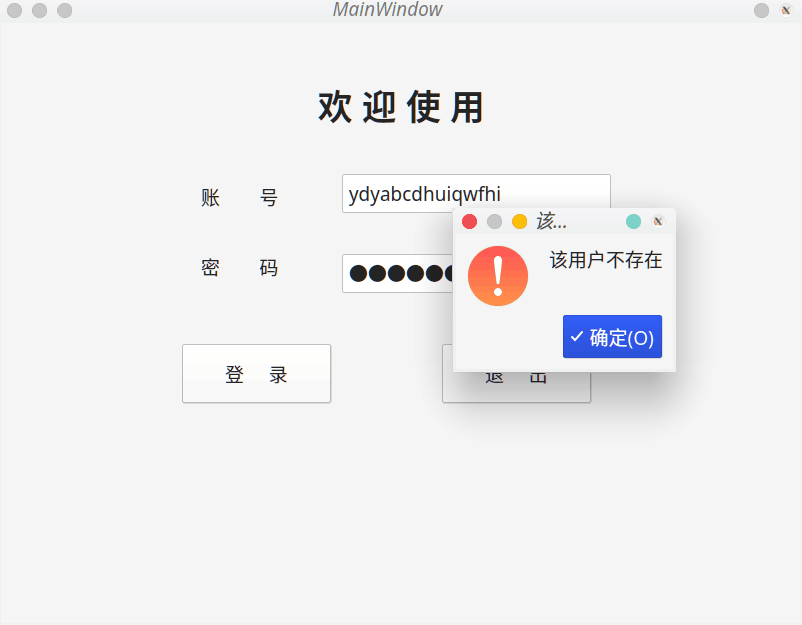
\includegraphics[width=1\columnwidth]{4.png}
	
}

当用户输入的账号错误时,系统提示“该用户不存在”。

{\centering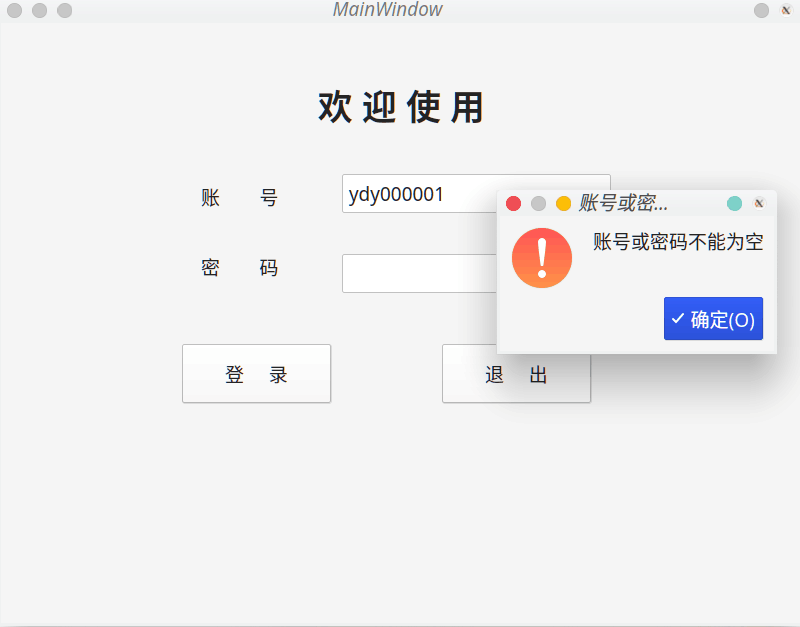
\includegraphics[width=1\columnwidth]{5.png}
	
}

当用户提交时尚未输入账号或密码时,系统提示“账号或密码不能为空”。

登录成功后,系统根据用户权限等级的不同,分别显示各用户对应的个人基本信息,并提供其权限等级所对应的功能选项。三种用户权限等级都含有“返回”和“退出”按钮,用于返回上一界面与退出系统。系统为三种用户权限等级都提供了基本信息修改功能,用户可以随时修改自己的个人基本信息。

{\centering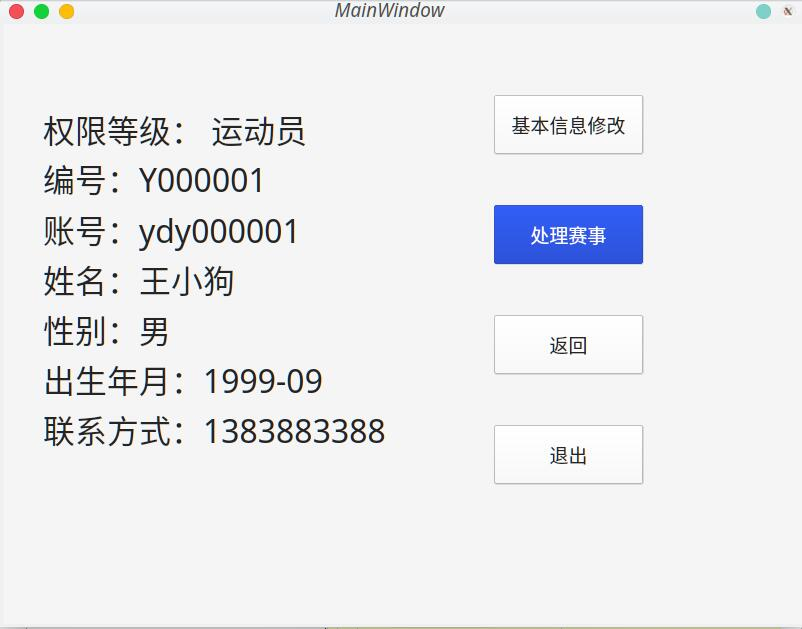
\includegraphics[width=1\columnwidth]{6.png}
	
}

运动员用户主页显示的基本信息包括权限等级、运动员编号、账号、姓名、性别、出生年月、联系方式。系统为运动员用户提供了处理赛事功能选项。

{\centering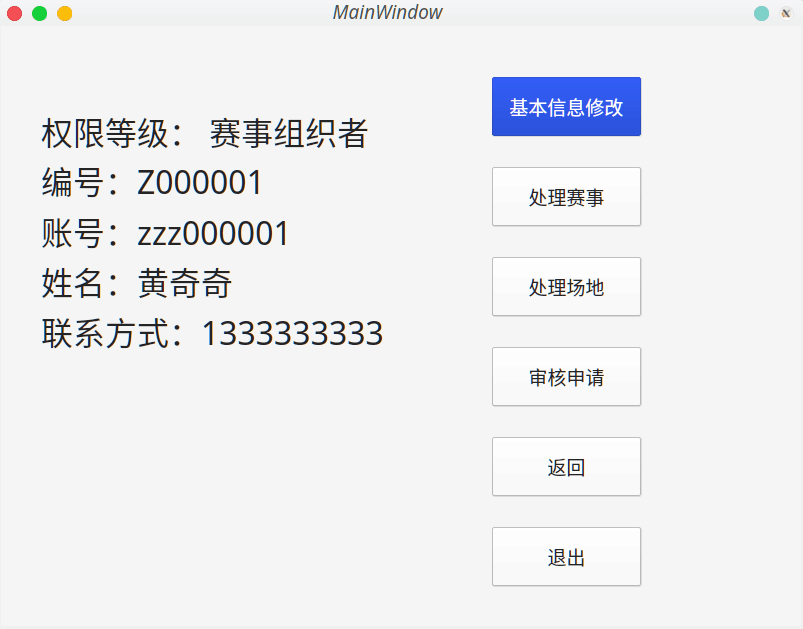
\includegraphics[width=1\columnwidth]{8.png}
	
}

赛事组织者用户主页显示的基本信息包括权限等级、赛事组织者编号、账号、姓名、联系方式。系统为赛事组织者用户提供了处理赛事、处理场地、审核申请三种功能选项。

{\centering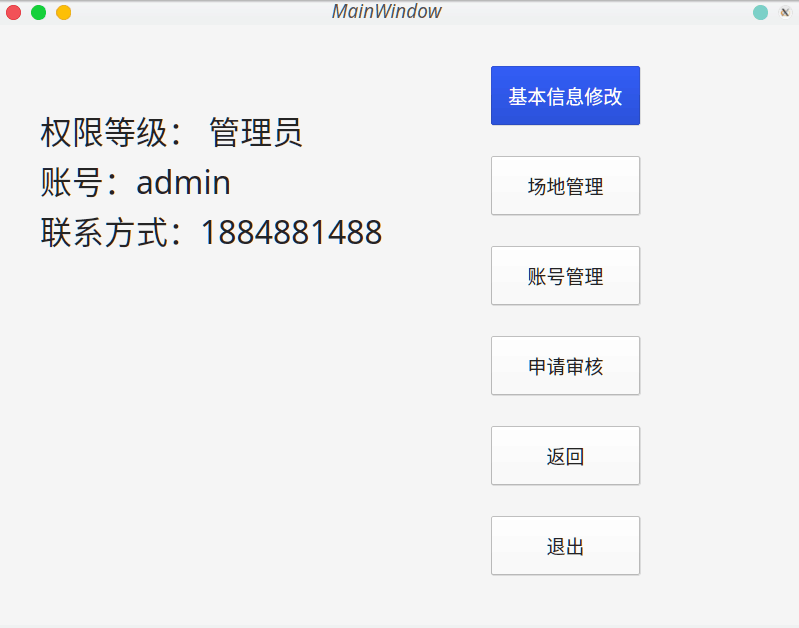
\includegraphics[width=1\columnwidth]{7.png}
	
}

管理员用户主页显示的基本信息包括权限等级、账号、联系方式。系统为赛事组织者用户提供了场地管理、账号管理、申请审核三种功能选项。

在主页选择某个功能选项后,若相应功能对应多个子功能,则跳转到对应的子功能选择界面,每个子功能选择界面都提供“返回”和“退出”按钮,用于返回上一界面与退出系统。子功能页面顶部显示该页面功能,如”赛事处理“、”场地处理“等,并显示当前用户的用户权限等级与用户编号。

{\centering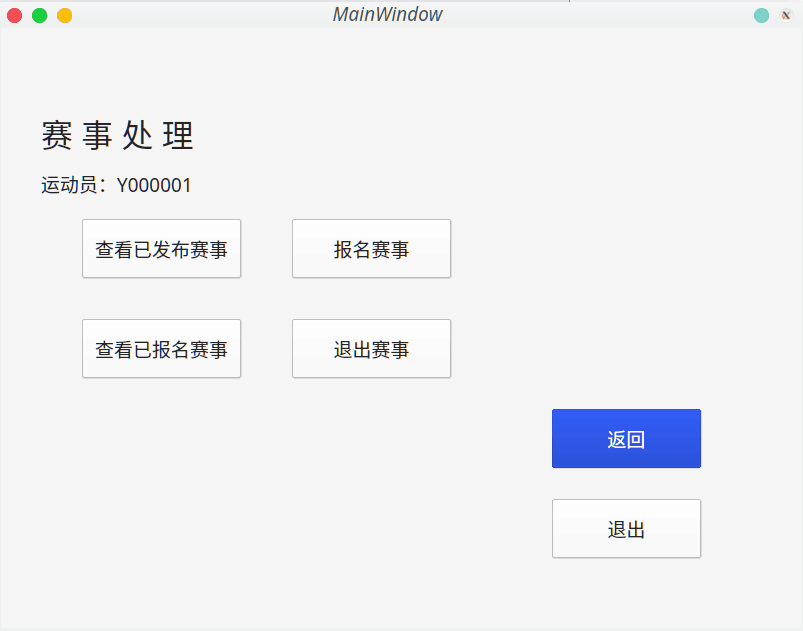
\includegraphics[width=1\columnwidth]{9.png}
	
}

上图为运动员权限下的”赛事处理“子功能选择界面,界面提供了“查看已发布赛事”、“报名赛事”、“查看已报名赛事”、“退出赛事”四个功能选项。

{\centering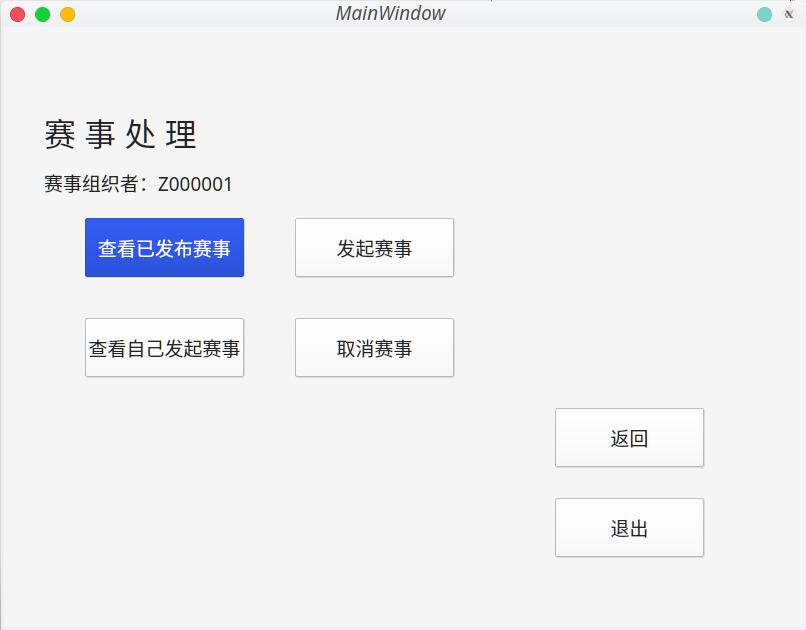
\includegraphics[width=1\columnwidth]{10.png}
	
}

上图为赛事组织者权限下的”赛事处理“子功能选择界面,界面提供了“查看已发布赛事”、“发起赛事”、“查看自己发起赛事”、“取消赛事”四个功能选项。

{\centering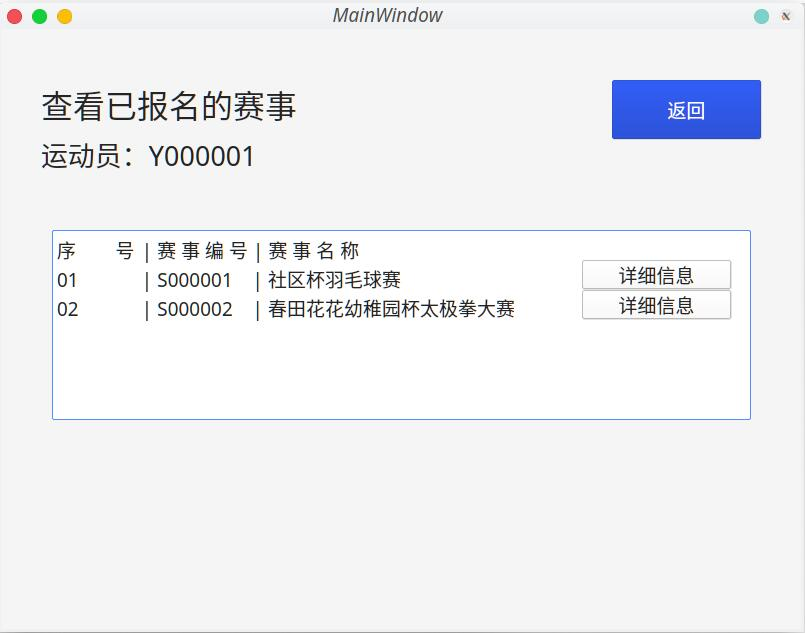
\includegraphics[width=1\columnwidth]{11.png}
	
}

“查看已发布的赛事”功能界面查询当前用户已成功报名的赛事,若未查询到结果,则提示“您当前尚未报名参与赛事”;若查询成功则返回并罗列查询结果,每一项查询结果仅包括赛事编号和赛事名称,用户可选择特定的结果项,点击最后的“详细信息”按钮查看其详细信息,详细信息仅包括赛事编号、赛事名称、赛事起止时间、赛事举办场地、赛事组织者姓名、赛事组织者联系方式、赛事说明以及赛事当前状态(预热中、进行中、已结束)。

{\centering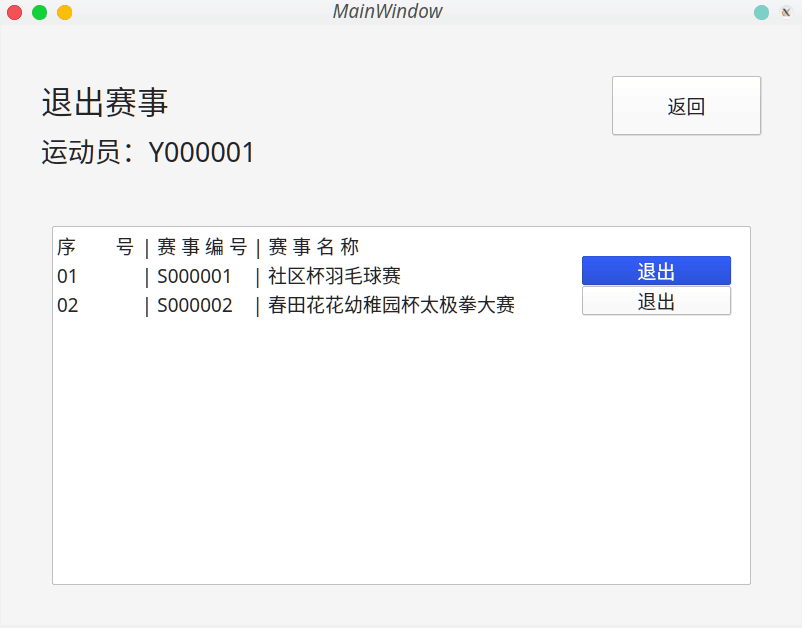
\includegraphics[width=1\columnwidth]{12.png}
	
}

“退出赛事”功能界面查询并罗列当前用户已成功报名的赛事。当赛事处于预热中状态时,用户点击每行数据项最后的“退出”按钮退出已报名的赛事。

{\centering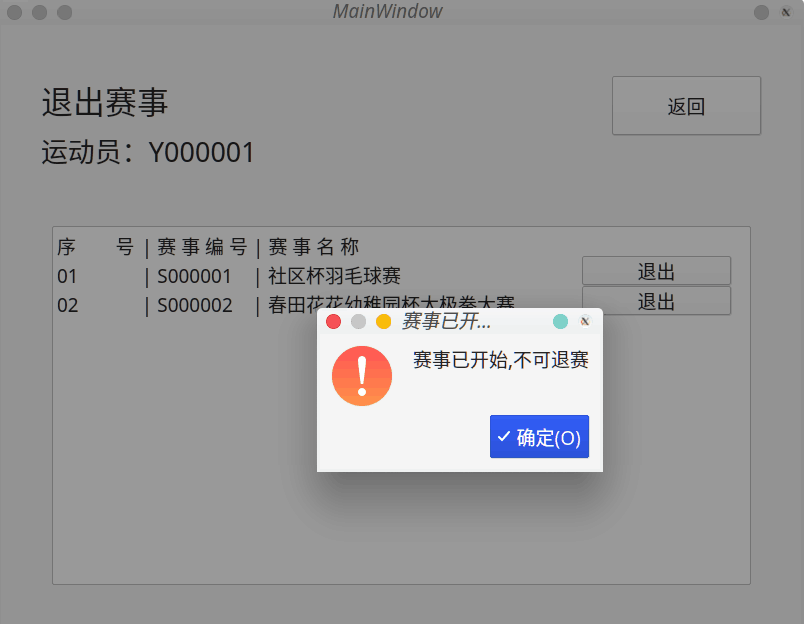
\includegraphics[width=1\columnwidth]{13.png}
	
}

赛事处于处于进行中状态,系统提示“赛事已开始,不可退赛”,退赛失败。

{\centering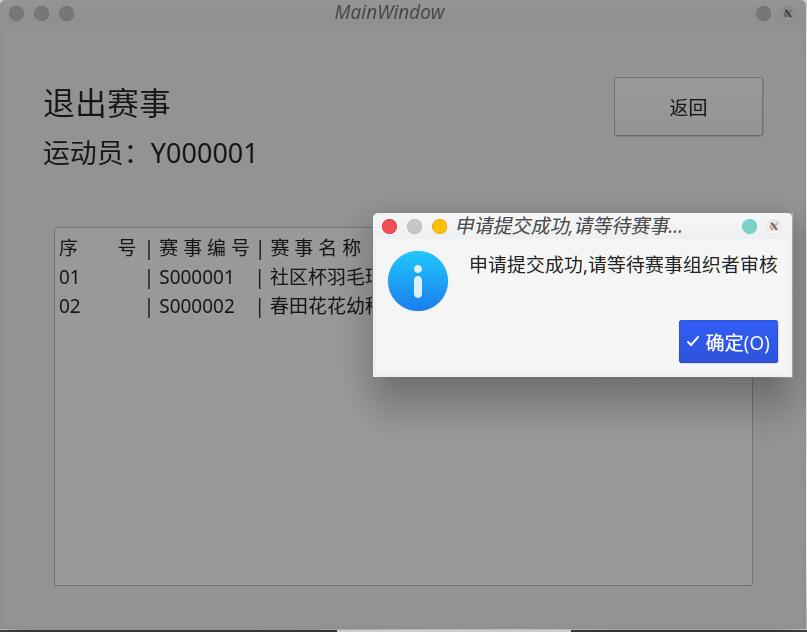
\includegraphics[width=1\columnwidth]{14.png}
	
}

退赛申请提交成功后,提示“申请提交成功,请等待赛事组织者审核”,并由系统交由赛事组织者进行审核,第一时间通过站内消息将审核结果通知给运动员。


{\centering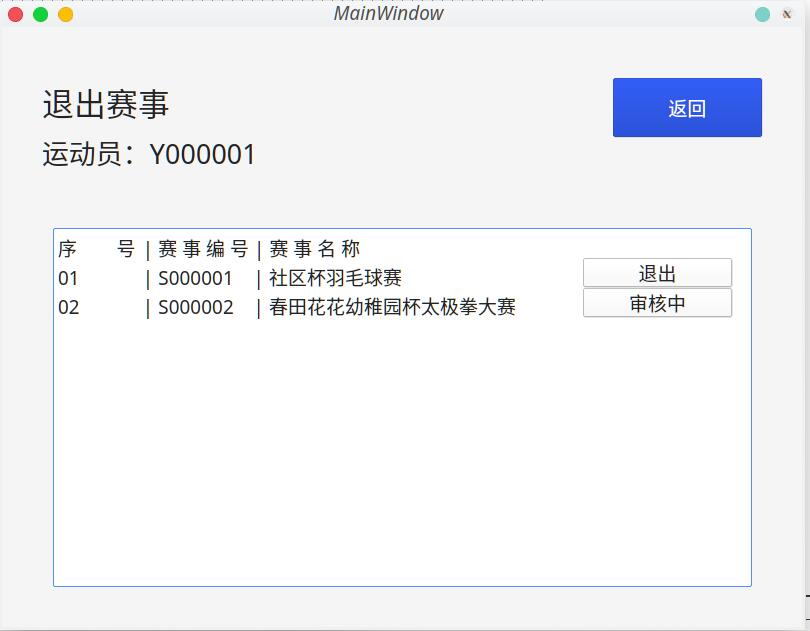
\includegraphics[width=1\columnwidth]{15.png}
	
}

退赛申请提交成功后,对应数据项最后的“退出”按钮变为“审核中”,并且变成失效状态,点击后没有相应。

{\centering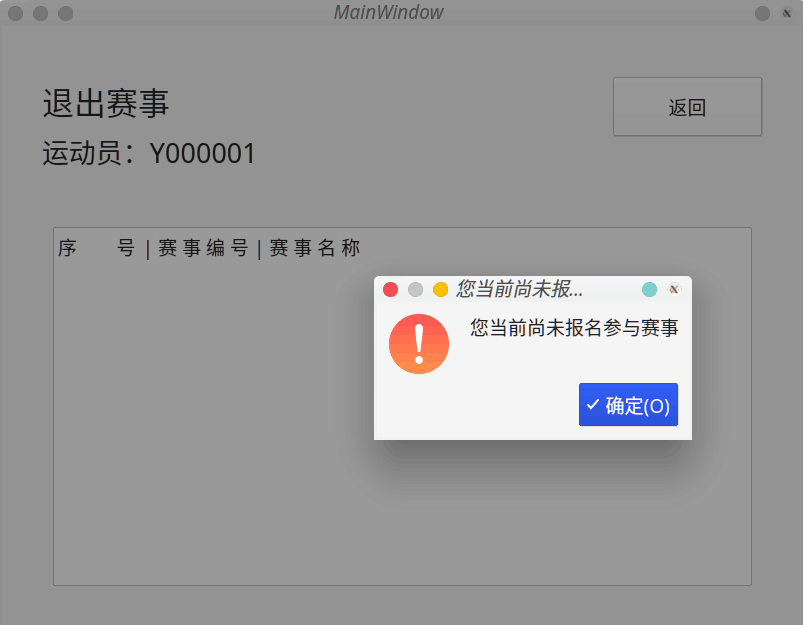
\includegraphics[width=1\columnwidth]{16.png}
	
}

若当前运动员用户尚未成功报名参与任何赛事,则提示“你当前尚未报名参与赛事”,点击“确定”后返回上一界面。

{\centering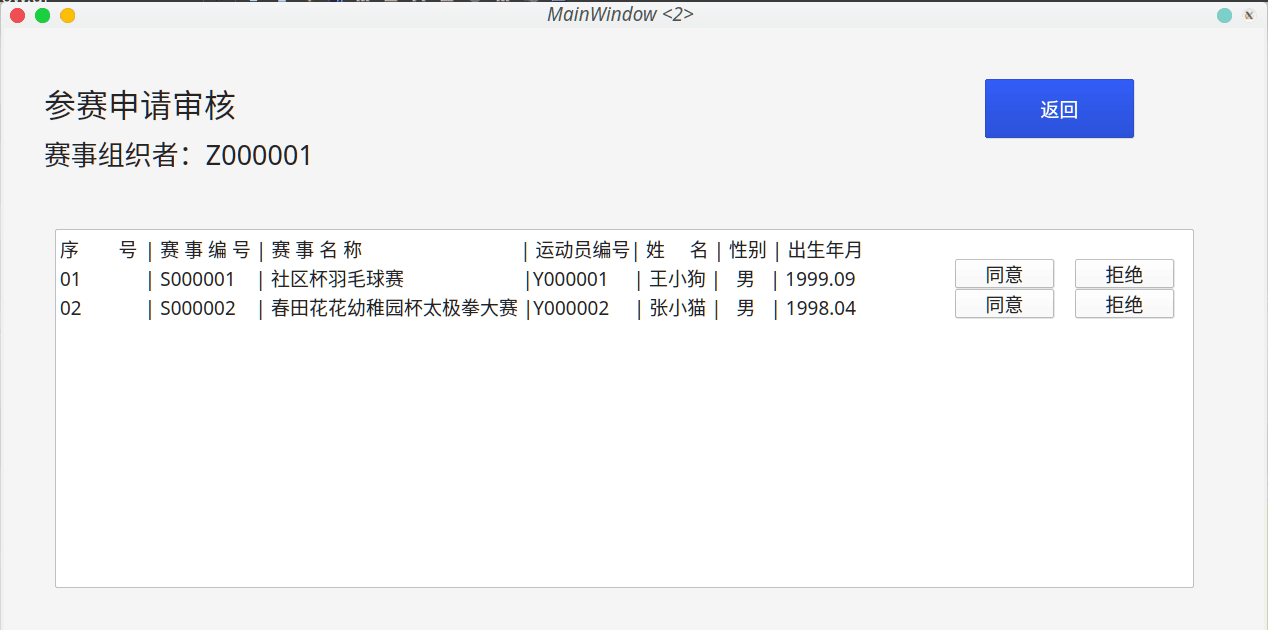
\includegraphics[width=1\columnwidth]{18.png}
	
}

“参赛申请审核”功能界面罗列待处理的参赛申请审核数据项,显示相应赛事的赛事编号、赛事名称,以及相应运动员的运动员编号、姓名、性别、出生年月,赛事组织者用户可以选择点击“同意”或“拒绝”按钮进行后提交,若选择拒绝,可以选择附加说明信息一同反馈给运动员。

{\centering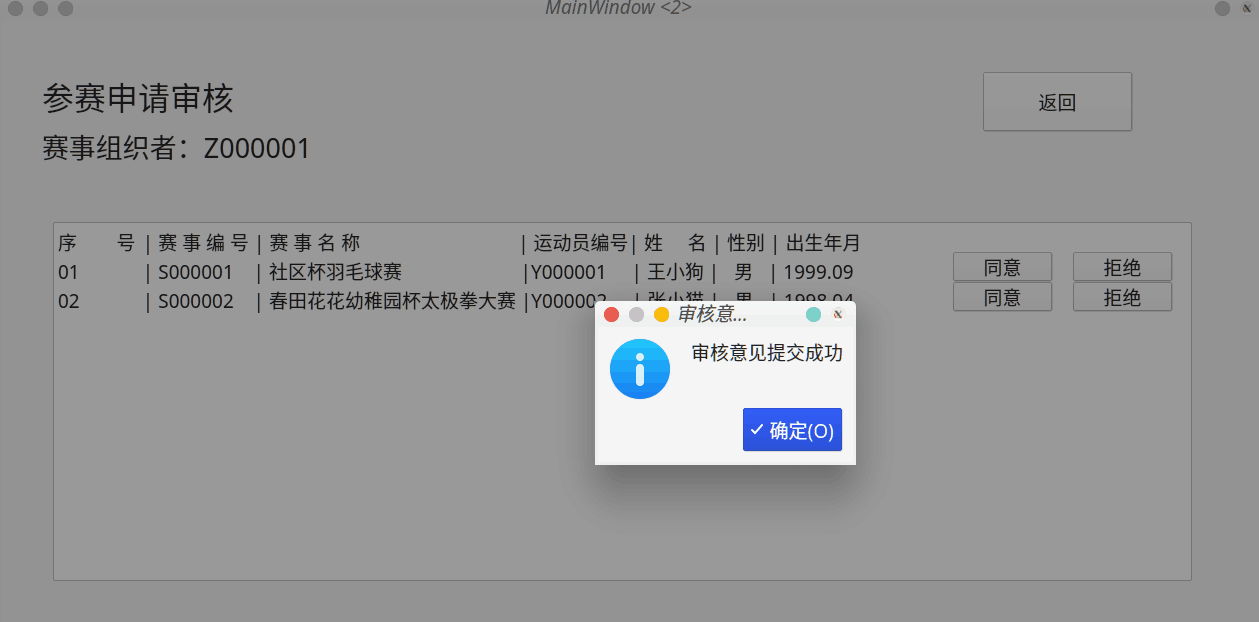
\includegraphics[width=1\columnwidth]{17.png}
	
}

提交成功后提示“审核意见提交成功”,点击“确定”后可继续审核其他申请,用户可以按“返回”按钮,返回到上一界面。

\section{总结}
本次项目实习开发了一个体育竞赛赛程与场地管理系统,可以为赛事组织者管理赛程和场地,并且让包括运动员在内的相关人员查看赛事情况。经过分析与设计建模、项目编码与测试,最终完成了系统的开发。

通过本次项目实习,熟悉了软件开发过程活动的主要内容,掌握了典型的软件过程组织模式,培养了针对项目特点具体应用、组织软件活动的能力;掌握了软件需求分析和设计的原理,能够采用正确的方法和思路建立分析和设计模型,基本掌握了为软件项目选择合适的平台予以实施的能力;能够初步理解软件验证的重要性,掌握了测试理论、方法和活动;掌握了软件项目管理的主要内容。

本次开环境为Manjaro Linux 20.0.1 Lysia + Windows 10 + Qt 5.12,报告撰写工具为LaTex + Visio。
	
\end{document}